% Options for packages loaded elsewhere
\PassOptionsToPackage{unicode}{hyperref}
\PassOptionsToPackage{hyphens}{url}
\documentclass[
]{article}
\usepackage{xcolor}
\usepackage[margin=1in]{geometry}
\usepackage{amsmath,amssymb}
\setcounter{secnumdepth}{5}
\usepackage{iftex}
\ifPDFTeX
  \usepackage[T1]{fontenc}
  \usepackage[utf8]{inputenc}
  \usepackage{textcomp} % provide euro and other symbols
\else % if luatex or xetex
  \usepackage{unicode-math} % this also loads fontspec
  \defaultfontfeatures{Scale=MatchLowercase}
  \defaultfontfeatures[\rmfamily]{Ligatures=TeX,Scale=1}
\fi
\usepackage{lmodern}
\ifPDFTeX\else
  % xetex/luatex font selection
\fi
% Use upquote if available, for straight quotes in verbatim environments
\IfFileExists{upquote.sty}{\usepackage{upquote}}{}
\IfFileExists{microtype.sty}{% use microtype if available
  \usepackage[]{microtype}
  \UseMicrotypeSet[protrusion]{basicmath} % disable protrusion for tt fonts
}{}
\makeatletter
\@ifundefined{KOMAClassName}{% if non-KOMA class
  \IfFileExists{parskip.sty}{%
    \usepackage{parskip}
  }{% else
    \setlength{\parindent}{0pt}
    \setlength{\parskip}{6pt plus 2pt minus 1pt}}
}{% if KOMA class
  \KOMAoptions{parskip=half}}
\makeatother
\usepackage{color}
\usepackage{fancyvrb}
\newcommand{\VerbBar}{|}
\newcommand{\VERB}{\Verb[commandchars=\\\{\}]}
\DefineVerbatimEnvironment{Highlighting}{Verbatim}{commandchars=\\\{\}}
% Add ',fontsize=\small' for more characters per line
\usepackage{framed}
\definecolor{shadecolor}{RGB}{248,248,248}
\newenvironment{Shaded}{\begin{snugshade}}{\end{snugshade}}
\newcommand{\AlertTok}[1]{\textcolor[rgb]{0.94,0.16,0.16}{#1}}
\newcommand{\AnnotationTok}[1]{\textcolor[rgb]{0.56,0.35,0.01}{\textbf{\textit{#1}}}}
\newcommand{\AttributeTok}[1]{\textcolor[rgb]{0.13,0.29,0.53}{#1}}
\newcommand{\BaseNTok}[1]{\textcolor[rgb]{0.00,0.00,0.81}{#1}}
\newcommand{\BuiltInTok}[1]{#1}
\newcommand{\CharTok}[1]{\textcolor[rgb]{0.31,0.60,0.02}{#1}}
\newcommand{\CommentTok}[1]{\textcolor[rgb]{0.56,0.35,0.01}{\textit{#1}}}
\newcommand{\CommentVarTok}[1]{\textcolor[rgb]{0.56,0.35,0.01}{\textbf{\textit{#1}}}}
\newcommand{\ConstantTok}[1]{\textcolor[rgb]{0.56,0.35,0.01}{#1}}
\newcommand{\ControlFlowTok}[1]{\textcolor[rgb]{0.13,0.29,0.53}{\textbf{#1}}}
\newcommand{\DataTypeTok}[1]{\textcolor[rgb]{0.13,0.29,0.53}{#1}}
\newcommand{\DecValTok}[1]{\textcolor[rgb]{0.00,0.00,0.81}{#1}}
\newcommand{\DocumentationTok}[1]{\textcolor[rgb]{0.56,0.35,0.01}{\textbf{\textit{#1}}}}
\newcommand{\ErrorTok}[1]{\textcolor[rgb]{0.64,0.00,0.00}{\textbf{#1}}}
\newcommand{\ExtensionTok}[1]{#1}
\newcommand{\FloatTok}[1]{\textcolor[rgb]{0.00,0.00,0.81}{#1}}
\newcommand{\FunctionTok}[1]{\textcolor[rgb]{0.13,0.29,0.53}{\textbf{#1}}}
\newcommand{\ImportTok}[1]{#1}
\newcommand{\InformationTok}[1]{\textcolor[rgb]{0.56,0.35,0.01}{\textbf{\textit{#1}}}}
\newcommand{\KeywordTok}[1]{\textcolor[rgb]{0.13,0.29,0.53}{\textbf{#1}}}
\newcommand{\NormalTok}[1]{#1}
\newcommand{\OperatorTok}[1]{\textcolor[rgb]{0.81,0.36,0.00}{\textbf{#1}}}
\newcommand{\OtherTok}[1]{\textcolor[rgb]{0.56,0.35,0.01}{#1}}
\newcommand{\PreprocessorTok}[1]{\textcolor[rgb]{0.56,0.35,0.01}{\textit{#1}}}
\newcommand{\RegionMarkerTok}[1]{#1}
\newcommand{\SpecialCharTok}[1]{\textcolor[rgb]{0.81,0.36,0.00}{\textbf{#1}}}
\newcommand{\SpecialStringTok}[1]{\textcolor[rgb]{0.31,0.60,0.02}{#1}}
\newcommand{\StringTok}[1]{\textcolor[rgb]{0.31,0.60,0.02}{#1}}
\newcommand{\VariableTok}[1]{\textcolor[rgb]{0.00,0.00,0.00}{#1}}
\newcommand{\VerbatimStringTok}[1]{\textcolor[rgb]{0.31,0.60,0.02}{#1}}
\newcommand{\WarningTok}[1]{\textcolor[rgb]{0.56,0.35,0.01}{\textbf{\textit{#1}}}}
\usepackage{longtable,booktabs,array}
\newcounter{none} % for unnumbered tables
\usepackage{calc} % for calculating minipage widths
% Correct order of tables after \paragraph or \subparagraph
\usepackage{etoolbox}
\makeatletter
\patchcmd\longtable{\par}{\if@noskipsec\mbox{}\fi\par}{}{}
\makeatother
% Allow footnotes in longtable head/foot
\IfFileExists{footnotehyper.sty}{\usepackage{footnotehyper}}{\usepackage{footnote}}
\makesavenoteenv{longtable}
\usepackage{graphicx}
\makeatletter
\newsavebox\pandoc@box
\newcommand*\pandocbounded[1]{% scales image to fit in text height/width
  \sbox\pandoc@box{#1}%
  \Gscale@div\@tempa{\textheight}{\dimexpr\ht\pandoc@box+\dp\pandoc@box\relax}%
  \Gscale@div\@tempb{\linewidth}{\wd\pandoc@box}%
  \ifdim\@tempb\p@<\@tempa\p@\let\@tempa\@tempb\fi% select the smaller of both
  \ifdim\@tempa\p@<\p@\scalebox{\@tempa}{\usebox\pandoc@box}%
  \else\usebox{\pandoc@box}%
  \fi%
}
% Set default figure placement to htbp
\def\fps@figure{htbp}
\makeatother
\setlength{\emergencystretch}{3em} % prevent overfull lines
\providecommand{\tightlist}{%
  \setlength{\itemsep}{0pt}\setlength{\parskip}{0pt}}
\usepackage{booktabs}
\usepackage{float}
\usepackage{amsmath}
\floatplacement{figure}{H}
\usepackage{booktabs}
\usepackage{longtable}
\usepackage{array}
\usepackage{multirow}
\usepackage{wrapfig}
\usepackage{float}
\usepackage{colortbl}
\usepackage{pdflscape}
\usepackage{tabu}
\usepackage{threeparttable}
\usepackage{threeparttablex}
\usepackage[normalem]{ulem}
\usepackage{makecell}
\usepackage{xcolor}
\usepackage{bookmark}
\IfFileExists{xurl.sty}{\usepackage{xurl}}{} % add URL line breaks if available
\urlstyle{same}
\hypersetup{
  pdftitle={Project 2: Modelling daily cycling demand in Edinburgh},
  pdfauthor={Group members: {[}Karthik Sutheeshkumar{]}, {[}Kiet Lam{]}, {[}Leon{]}},
  hidelinks,
  pdfcreator={LaTeX via pandoc}}

\title{Project 2: Modelling daily cycling demand in Edinburgh}
\author{Group members: {[}Karthik Sutheeshkumar{]}, {[}Kiet Lam{]}, {[}Leon{]}}
\date{Word count: {[}0 words{]}}

\begin{document}
\maketitle

\section{Introduction}\label{introduction}

Edinburgh operates a network of automatic cycling counters at strategic locations across the city that records the total number of cyclists passing each site daily, The resulting dataset contains 2,180 observations spanning from 2020 to 2025, covering a period that includes the COVID-19 pandemic and a gradual return to normal travel patterns. Using this data, we evaluate a sequence of linear regression models of increasing complexity rigorously to explain how daily cycling demand varies with weather conditions, day of week, seasonality, and longer-term trend, evaluating each model using leave-one-year-out cross validation. The analysis is guided by three questions of practical interest to Edinburgh City Council: how well the model predicts demand across different seasons, how sensitive cycling is to temperature, and what the long-term trend implies for infrastructure planning over the next decade.

\section{Exploratory data analysis}\label{exploratory-data-analysis}

Three derived variables are created before modelling. First, month is converted
to an ordered factor with levels 1--12, ensuring plots display January to December
in the correct order. Second, day of week is re-specified with explicit levels
from Sunday to Saturday, overriding R's default alphabetical ordering. Third,
a numeric trend variable is derived as the integer number of days elapsed since
1 January 2020, so that trend = 0 corresponds to the start of the observation
period and increases by 1 for each subsequent day. This allows the model to
capture any linear drift in cycling demand over 2020--2025.

\begin{table}

\caption{\label{tab:unnamed-chunk-1}Summary statistics for daily cyclist count and temperature variables.}
\centering
\begin{tabular}[t]{lrrrrr}
\toprule
Variable & Mean & SD & Min & Median & Max\\
\midrule
Daily Count & 10815.5 & 4728.9 & 1264.0 & 10531.0 & 43864\\
Mean Temp (°C) & 9.7 & 4.8 & -8.1 & 9.8 & 23\\
Min Temp (°C) & 5.9 & 5.0 & -14.0 & 6.0 & 18\\
Max Temp (°C) & 13.2 & 5.3 & -3.0 & 13.0 & 31\\
\bottomrule
\end{tabular}
\end{table}

Table 1 summarises the key numeric variables across the 2180 daily observations. Daily cyclist count average around 10,816 but with a large standard deviation of 4729 reflecting strong seasonal variation. The minimum and maximum count of 1,264 and 43,864 respectively confirm that demand varies dramatically across the year. Edinburgh's climate is characterized by mild but cool conditions, with mean daily temperatures averaging 9.7°C and ranging from -8.1°C to 23°C, typical for a Scottish city. The wide spread in temperature variables, ranging from -14°C to 31°C, suggests that weather conditions vary considerably across the observation period and are likely to play an important role in explaining day-to-day variation in cycling demand.

\begin{figure}
\centering
\pandocbounded{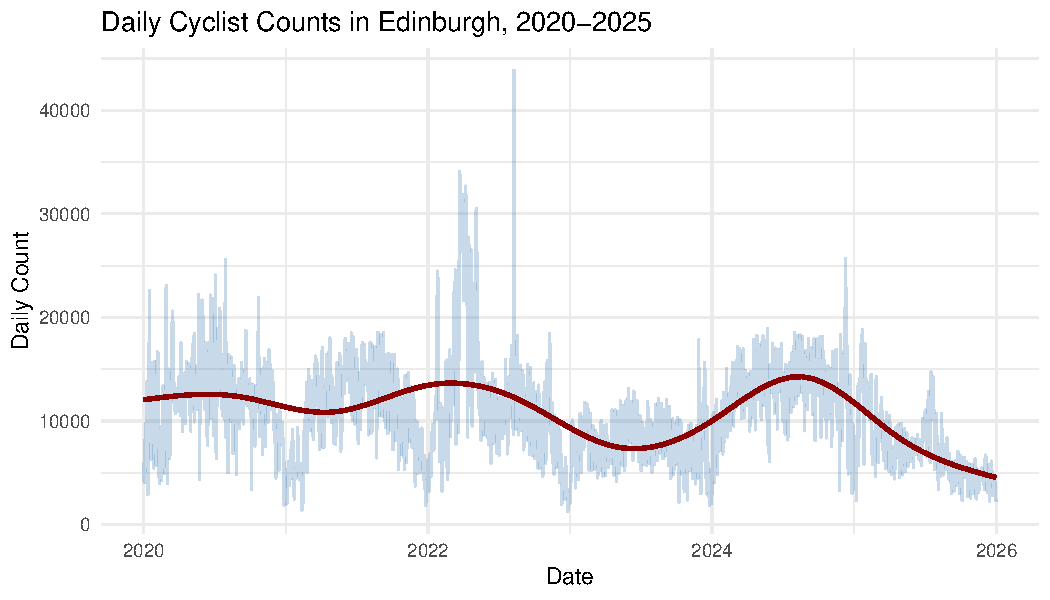
\includegraphics[keepaspectratio,alt={\label{fig:fig-ts} Time series of daily cyclist counts in Edinburgh (2020--2025) with a smoother.}]{Report_project02-1----3000_files/figure-latex/fig-ts-1.pdf}}
\caption{\label{fig:fig-ts} Time series of daily cyclist counts in Edinburgh (2020--2025) with a smoother.}
\end{figure}

Figure \ref{fig:fig-ts} shows the daily cyclist counts across the full observation period from 2020-2025, with a smoother overlaid to highlight the trend, filtering out day-to-day variability. We can see the obvious pattern that the daily count climbs every summer and fall back each winter, and this repeats every year. There is a visible dip around 2020-2021, which is unsurprising given the COVID-19 lockdowns during that period. After that, daily counts reach their highest levels around 2022-23. The drop at the end of the observation period coincides with the data ending in early 2026, making it difficult to distinguish a seasonal effect from a genuine trend change. Certain days stands out in count, especially one around 2022 that exceeds 40,000 cyclists a day, which probably reflects an unusually warm day.

\textbf{Boxplots of count by month and by day of week }

\begin{figure}
\centering
\pandocbounded{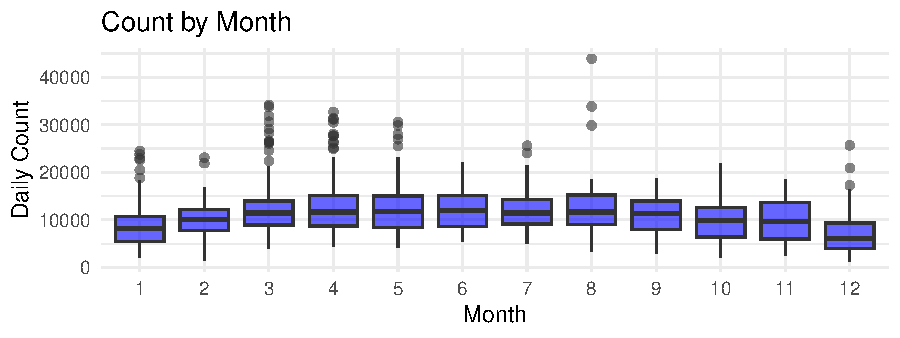
\includegraphics[keepaspectratio,alt={\label{fig:fig-boxplotmonth}Distribution of daily cyclist counts by month.}]{Report_project02-1----3000_files/figure-latex/fig-boxplotmonth-1.pdf}}
\caption{\label{fig:fig-boxplotmonth}Distribution of daily cyclist counts by month.}
\end{figure}

Figure \ref{fig:fig-boxplotmonth} confirms the seasonal pattern seen in the time series. Counts are lowest in January and December, with medians around 10,500-11,500 cyclists per day, rising steadily through spring and peaking between May and August. Winter months see roughly half the cycling activity of summer months, which has clear implications for seasonal infrastructure planning.

\begin{figure}
\centering
\pandocbounded{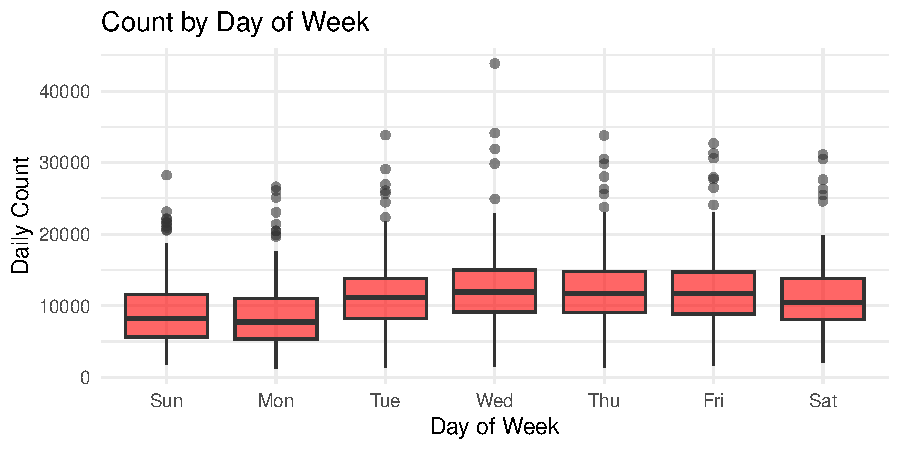
\includegraphics[keepaspectratio,alt={\label{fig:fig-boxplotdow}Distribution of daily cyclist counts by day of week}]{Report_project02-1----3000_files/figure-latex/fig-boxplotdow-1.pdf}}
\caption{\label{fig:fig-boxplotdow}Distribution of daily cyclist counts by day of week}
\end{figure}

Figure \ref{fig:fig-boxplotdow} suggests that cycling demand is higher on weekdays than weekends, with Tuesday to Friday showing the highest medians of around 11,000-12,000 cyclists per day. Sunday and Monday stand out as the lowest, with medians closer to 8,000-9,000, suggesting that commuting is a major driver of cycling demand in Edinburgh.

\textbf{Scatter plot of count vs temp\_mean}

\begin{figure}
\centering
\pandocbounded{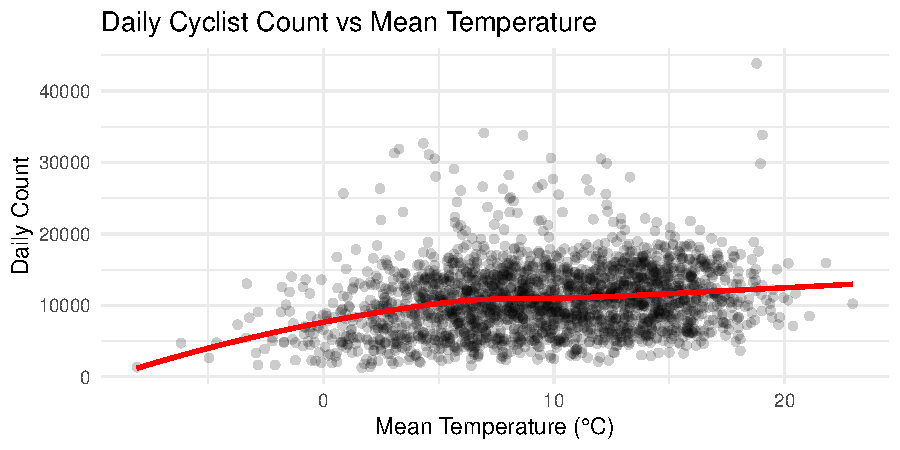
\includegraphics[keepaspectratio,alt={\label{fig:fig-scattertemp}Daily cyclist count versus mean temperature}]{Report_project02-1----3000_files/figure-latex/fig-scattertemp-1.pdf}}
\caption{\label{fig:fig-scattertemp}Daily cyclist count versus mean temperature}
\end{figure}

Figure \ref{fig:fig-scattertemp} shows a clear positive but non-linear relationship between mean temperature and daily cyclist counts. Counts rise steeply at lower temperatures before leveling off above around 10--12°C, suggesting a quadratic relationship for temperature term. The spread of counts also increases with temperature, suggesting heteroscedasticity.

\textbf{Showing relation between count and mean temperature during COVID and post COVID period}

\begin{figure}
\centering
\pandocbounded{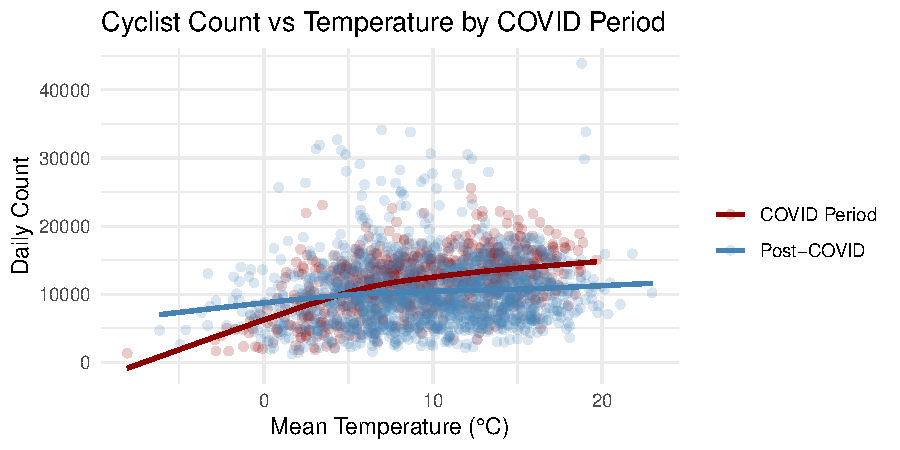
\includegraphics[keepaspectratio,alt={\label{fig:fig-covidscatter}Daily cyclist count versus mean temperature by COVID and post-COVID period (2020--2025)}]{Report_project02-1----3000_files/figure-latex/fig-covidscatter-1.pdf}}
\caption{\label{fig:fig-covidscatter}Daily cyclist count versus mean temperature by COVID and post-COVID period (2020--2025)}
\end{figure}

Figure \ref{fig:fig-covidscatter} reveals an interesting and somewhat counter intuitive pattern --- cycling counts during the COVID period (2020-2021) were actually higher at warmer temperatures compared to post-COVID years, with the red smoother sitting well
above the blue at temperatures above 10°C. This likely reflects that during the covid lockdowns, cycling shifted from commuting to recreational use, with people more willing to cycle on pleasant days but much less likely to cycle in cold or wet
conditions, explaining the steeper temperature sensitivity. At cold temperatures the pattern reverses, with post-COVID counts higher, consistent with commuters cycling regardless of weather. This difference in behaviour between the two periods suggests that a COVID indicator variable may improve model fit, and motivates its inclusion as a candidate extension in M3.

\section{Baseline model M0}\label{baseline-model-m0}

In all of the models that we will fit, the response variable is \(y_i = \text{count}_i\), the total
daily cyclist count on date \(i\), for each day \(i\) from 1 January 2020 to 31 December
2025. Four models of increasing complexity are considered: M0 (baseline with numeric
month), M1 (adds linear trend and factor covariates), M2 (replaces linear temperature
with a quadratic term), and M3 (log-transforms the response to address non-normality).
The common predictors across all models are defined as follows:

\begin{align*}
x_{1i} &= \text{temp\_mean}_i \quad \text{(daily mean air temperature in °C)} \\
x_{2i} &= \text{weekend}_i \quad \text{(binary indicator: 1 if Saturday or Sunday, 0 otherwise)} \\
m_i &\in \{1, \ldots, 12\} \quad \text{(month: numeric in M0, factor in M1--M3)} \\
t_i &= \text{trend}_i \quad \text{(integer days since 2020-01-01, where $t_i = 0$ on 1 January 2020)} \\
d_i &= \text{dow}_i \quad \text{(day of week factor, reference level: Sunday)}
\end{align*}
All models assume \(\varepsilon_i \sim N(0, \sigma^2)\).

The baseline model M0, fitted for each day \(i\) from 1 January 2020 to
31 December 2025, is specified as:

\[
y_i = \beta_0 + \beta_1 x_{1i} + \beta_2 x_{2i} + \beta_3 m_i + \varepsilon_i, 
\quad \varepsilon_i \sim N(0, \sigma^2)
\]

\begin{table}

\caption{\label{tab:unnamed-chunk-2}Coefficients table for baseline model M0.}
\centering
\begin{tabular}[t]{lrrrr}
\toprule
term & estimate & std.error & statistic & p.value\\
\midrule
(Intercept) & 10385.819 & 267.015 & 38.90 & 0\\
temp\_mean & 247.179 & 20.769 & 11.90 & 0\\
weekend & -1246.888 & 214.172 & -5.82 & 0\\
month\_num & -247.184 & 28.810 & -8.58 & 0\\
\bottomrule
\end{tabular}
\end{table}

Table 2 shows the estimated coefficients for M0. All four predictors are highly significant \((p < 0.001)\). Each 1°C increase in mean temperature is associated with approximately 247 additional cyclists per day with the other variables held fixed, while weekend days see around 1,247 fewer cyclists than weekdays, consistent with the commuter-driven pattern observed
in the EDA. The negative month coefficient (-247) implies that daily count declines on average as the month increases, though this is a crude approximation since the relationship between month and demand is not linear.

\begin{figure}
\centering
\pandocbounded{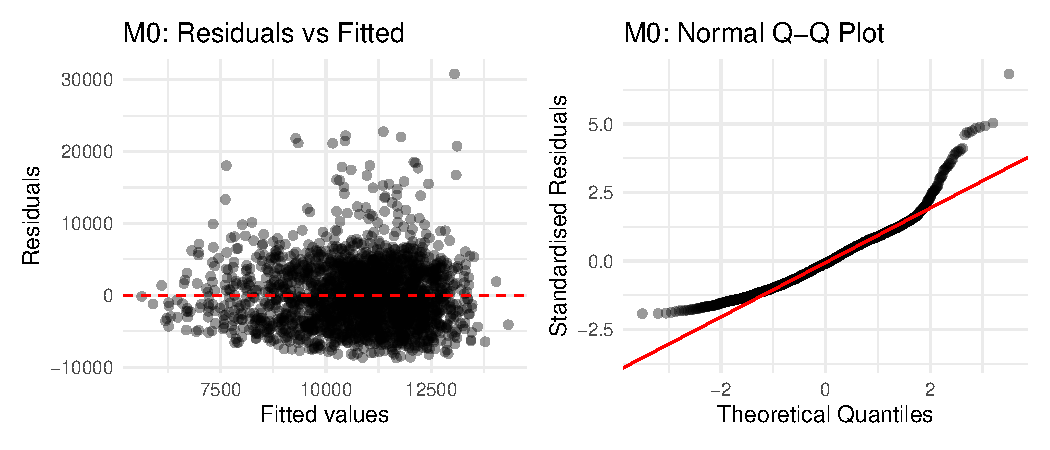
\includegraphics[keepaspectratio,alt={\label{fig:fig-m0diagnostics}Diagnostics for M0}]{Report_project02-1----3000_files/figure-latex/fig-m0diagnostics-1.pdf}}
\caption{\label{fig:fig-m0diagnostics}Diagnostics for M0}
\end{figure}

The residuals versus fitted plot shows that the spread of residuals grows
noticeably with fitted values, indicating heteroscedasticity --- a violation
of the constant variance assumption. The QQ plot reveals a heavy right tail, with standardized residuals curving sharply above the reference line at high quantiles, reflecting the right-skewed distribution typical of non-negative count data. Both issues suggest that M0's Gaussian assumption is inadequate.

M0 captures the broad direction of key predictors --- temperature, weekend effect, and seasonality but treats month as numeric, forcing a linear relationship across months that does not reflect the true seasonal pattern seen in the EDA. It also omits day of week entirely and includes no long-term trend. These limitations motivate M1, which switches month to a factor, adds day of week as a factor, and introduces a linear trend term to capture drift in cycling demand over 2020--2025.

\section{Proposed models M1--M3}\label{proposed-models-m1m3}

\subsection{Model M1: Trend and factor}\label{model-m1-trend-and-factor}

Model M1, fitted for each day \(i\) from 1 January 2020 to 31 December 2025,
is specified as:

\[
y_i = \beta_0 + \beta_1 x_{1i} + \beta_2 x_{2i} + \beta_3 t_i
+ \sum_{m=2}^{12} \gamma_m \mathbf{1}(m_i = m) 
+ \sum_{d=2}^{7} \delta_d \mathbf{1}(d_i = d) 
+ \varepsilon_i, \quad \varepsilon_i \sim N(0, \sigma^2)
\]

M1 extends M0 in three ways. First, month is switched from a numeric
predictor to a factor, giving each month its own intercept. Figure
\ref{fig:fig-boxplotmonth} shows that the month--demand relationship
is not monotonic, so forcing a single slope as M0 does is inappropriate.
Second, day of week is added as a factor --- the weekend binary in M0
groups Saturday and Sunday together, but Figure
\ref{fig:fig-boxplotdow} shows these days behave differently, so a
full factor allows each day its own effect. Third, a linear trend term
\(t_i\) is added to capture the drift in underlying demand visible in
Figure \ref{fig:fig-ts}. Both factors use dummy variable encoding with
January and Sunday as reference categories, so \(\gamma_m\) and \(\delta_d\)
represent differences relative to these baselines, and the sums begin
at \(m = 2\) and \(d = 2\) as the first level of each factor is absorbed
into \(\beta_0\).

\textbf{Diagnostics of M1}

\begin{figure}
\centering
\pandocbounded{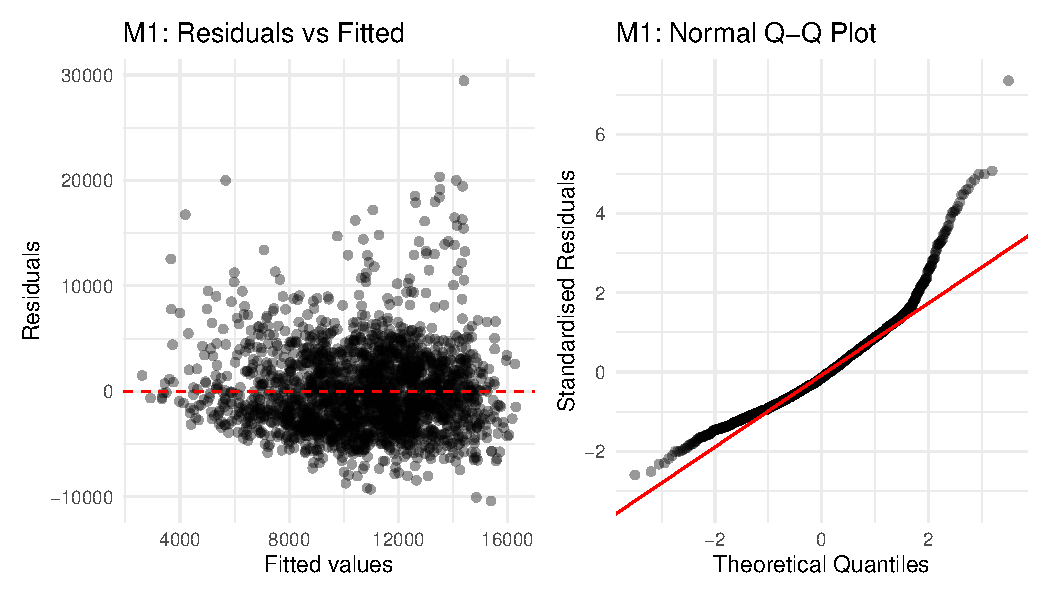
\includegraphics[keepaspectratio,alt={\label{fig:fig-m1diagnostics}Diagnostics for M1}]{Report_project02-1----3000_files/figure-latex/fig-m1diagnostics-1.pdf}}
\caption{\label{fig:fig-m1diagnostics}Diagnostics for M1}
\end{figure}

Compared to M0, M1 shows some improvement --- the fitted values span a wider range, suggesting the additional predictors (trend, factor month, factor day of week) give the model more flexibility to capture variation in demand. However, the core issues persist. The residuals versus fitted plot still shows increasing spread at higher fitted values, indicating that heteroscedasticity remains unresolved. The QQ plot continues to show a pronounced right tail, with standardized residuals reaching above 6 at the upper end, reflecting the right-skewed nature of the count data that a Gaussian model struggles to accommodate. These issues motivate further extensions in M2 and M3.

\subsection{Model M2: Nonlinear temperature}\label{model-m2-nonlinear-temperature}

Model M2, fitted for each day \(i\) from 1 January 2020 to 31 December 2025,
is specified as:

\[
y_i = \beta_0 + \beta_1 x_{1i} + \beta_2 x_{1i}^2 + \beta_3 x_{2i} + \beta_4 t_i
+ \sum_{m=2}^{12} \gamma_m \mathbf{1}(m_i = m) 
+ \sum_{d=2}^{7} \delta_d \mathbf{1}(d_i = d) 
+ \varepsilon_i, \quad \varepsilon_i \sim N(0, \sigma^2)
\]

M2 extends M1 by replacing the linear temperature term with a quadratic, adding both \(x_{1i}\) and \(x_{1i}^2\) as predictors. Figure \ref{fig:fig-scattertemp} shows that the temperature--demand relationship flattens above around 10°C, which a linear term cannot capture. The quadratic term allows the model to reflect this diminishing sensitivity, which is also physically plausible --- once conditions are warm enough, further temperature increases have a smaller effect on cycling behaviour.

\begin{figure}
\centering
\pandocbounded{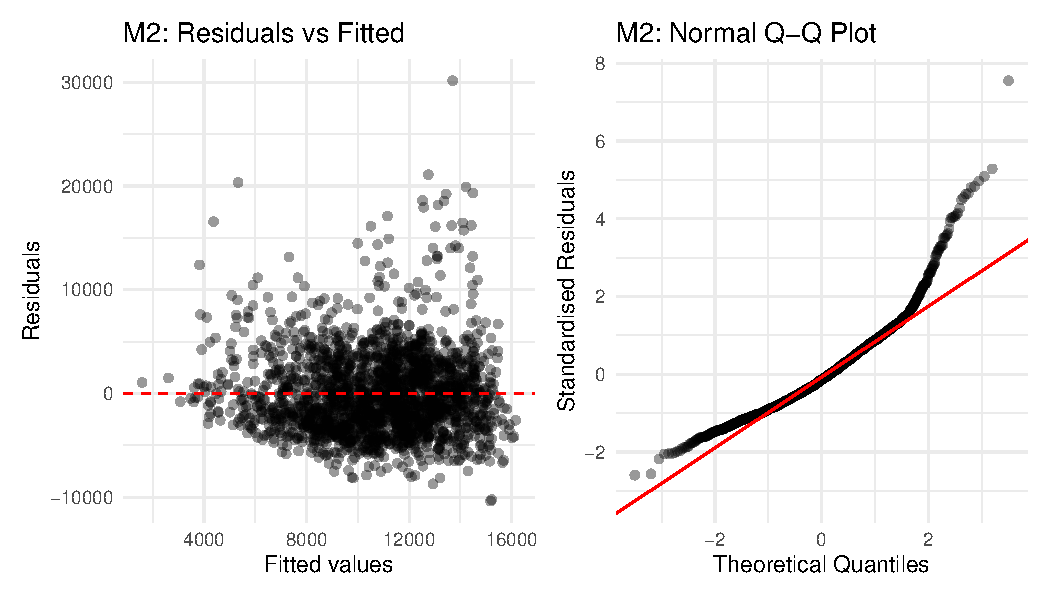
\includegraphics[keepaspectratio,alt={\label{fig:fig-m2diagnostics}Diagnostics for M2}]{Report_project02-1----3000_files/figure-latex/fig-m2diagnostics-1.pdf}}
\caption{\label{fig:fig-m2diagnostics}Diagnostics for M2}
\end{figure}

M2 shows marginal improvement over M1 --- residual spread is slightly more even and the lower QQ tail follows the reference line more closely. However, the right tail worsens, with standardised residuals exceeding 7, and heteroscedasticity persists. The consistently heavy right tail across M0, M1, and M2 suggests a Gaussian model is fundamentally inappropriate for the given data, motivating the log transformation in M3.

\subsection{Model M3: Log-Transformed Response}\label{model-m3-log-transformed-response}

Model M3, fitted for each day \(i\) from 1 January 2020 to 31 December 2025,
is specified as:

\[
\log(y_i + 1) = \beta_0 + \beta_1 x_{1i} + \beta_2 x_{1i}^2 + \beta_3 x_{2i} + \beta_4 t_i
+ \sum_{m=2}^{12} \gamma_m \mathbf{1}(m_i = m) 
+ \sum_{d=2}^{7} \delta_d \mathbf{1}(d_i = d) 
+ \varepsilon_i, \quad \varepsilon_i \sim N(0, \sigma^2)
\]

M3 keeps all predictors from M2 but log-transforms the response, fitting \(\log(\text{count}_i + 1)\) rather than \(\text{count}_i\) directly. The persistent right-skew and heteroscedasticity seen across M0--M2 are classic symptoms of modelling non-negative count data with a Gaussian assumption.The log transformation addresses this by compressing large values, reducing
skewness and stabilising variance. The \(+1\) ensures the transformation is defined if any zero counts are present.

\begin{figure}
\centering
\pandocbounded{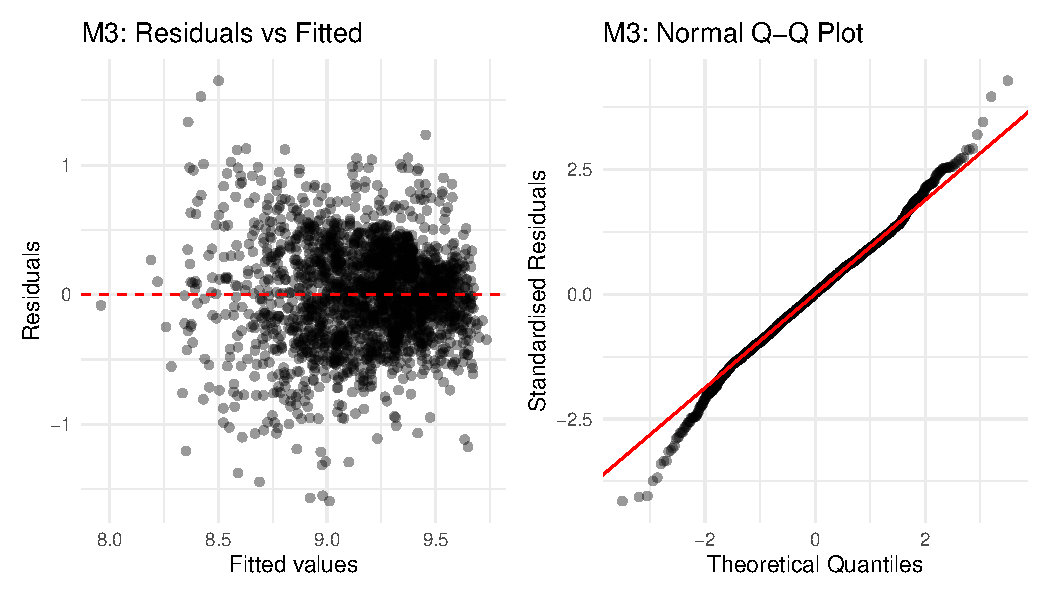
\includegraphics[keepaspectratio,alt={\label{fig:fig-m3diagnostics}Diagnostics for M3}]{Report_project02-1----3000_files/figure-latex/fig-m3diagnostics-1.pdf}}
\caption{\label{fig:fig-m3diagnostics}Diagnostics for M3}
\end{figure}

The diagnostic plots for M3 show a marked improvement --- residuals are now scattered evenly around zero and the QQ plot follows the reference line closely across almost its entire range, compared to the severe right tail deviation in M2. Some deviation remains at both tails, indicating slight remaining non-normality, but the Gaussian assumption is considerably more plausible for M3 than any earlier model.

\section{Evaluation}\label{evaluation}

\subsection{Statistical Performance}\label{statistical-performance}

\begin{table}[!h]
\centering
\caption{\label{tab:tab-cv1}Leave-one-year-out cross-validation scores for models M0--M3. Lower is better for all scores.}
\centering
\begin{tabular}[t]{lrrrr}
\toprule
model & RMSE & MAE & DS & IS\\
\midrule
M0 & 4740.9 & 3805.6 & 18.05 & 25630.5\\
M1 & 4602.3 & 3665.3 & 18.08 & 25391.0\\
M2 & 4587.6 & 3650.2 & 18.07 & 25277.9\\
M3 & 4530.8 & 3598.5 & 18.65 & 30353.6\\
\bottomrule
\end{tabular}
\end{table}

Table \ref{tab:tab-cv1} shows the CV scores across all four models. RMSE and MAE improve consistently from M0 to M3, with M3 achieving the lowest values of 4531 and 3598 respectively. However, M0 achieves the lowest DS (18.0) and M3 the highest (18.5), with M3 also notably worse on IS. This disagreement arises because back-transforming M3's log-scale predictions inflates predictive variance via the delta method, penalising DS and IS. M3 is nonetheless selected as the final model --- it achieves the best RMSE and MAE and is the only model whose diagnostic plots satisfy the normality and constant variance assumptions.

\begin{table}[!h]
\centering
\caption{\label{tab:tab-cv2}Monthly cross-validated RMSE and Dawid--Sebastiani score for the final model M3.}
\centering
\begin{tabular}[t]{lrr}
\toprule
Month & RMSE & DS\\
\midrule
Jan & 4377.6 & 18.16\\
Feb & 3973.2 & 17.79\\
Mar & 5886.6 & 18.77\\
Apr & 6485.7 & 19.34\\
May & 5035.7 & 18.27\\
\addlinespace
Jun & 3909.0 & 17.85\\
Jul & 3485.3 & 17.52\\
Aug & 5301.0 & 18.43\\
Sep & 4270.3 & 18.20\\
Oct & 4086.3 & 18.56\\
\addlinespace
Nov & 4310.5 & 18.59\\
Dec & 4381.3 & 22.27\\
\bottomrule
\end{tabular}
\end{table}

Table \ref{tab:tab-cv2} shows that predictive performance varies across the year. RMSE is lowest in July (3485.3) and highest in April (6485.7) and March (5886.6), suggesting early spring is hardest to predict. December has the worst DS (0.92), indicating poorer uncertainty calibration around that period. Early spring and December therefore present the greatest challenge for the final model.

\subsection{Practical Performance}\label{practical-performance}

\subsubsection{Temperature effects and nonlinearity}\label{temperature-effects-and-nonlinearity}

\begin{table}[!h]
\centering
\caption{\label{tab:tab-tempcompare}Comparison of nonlinear temperature specifications in the M2 model family.}
\centering
\begin{tabular}[t]{lrrr}
\toprule
temp\_var & RMSE & DS & IS\\
\midrule
temp\_max & 4599.1 & 18.09 & 25317.1\\
temp\_mean & 4587.6 & 18.07 & 25277.9\\
temp\_min & 4574.7 & 18.06 & 25010.3\\
\bottomrule
\end{tabular}
\end{table}

Table \ref{tab:tab-tempcompare} compares three nonlinear temperature specifications. \texttt{temp\_min} performs best with the lowest RMSE (4574.7)
and IS (25010.3), though DS is effectively identical across all three (difference of 0.03 at most). This is physically plausible --- commuters are more likely to base cycling decisions on the coldest conditions of the day, making minimum temperature the most behaviourally relevant measure.

\begin{table}[!h]
\centering
\caption{\label{tab:tab-tempeffect}Estimated marginal effect of a 1°C increase using the chosen temperature variable.}
\centering
\begin{tabular}[t]{lr}
\toprule
Temperature & Marginal.effect..cyclists.per..1C.\\
\midrule
5C & 53.9\\
15C & -250.2\\
\bottomrule
\end{tabular}
\end{table}

Table \ref{tab:tab-tempeffect} shows the marginal effects for the chosen specification. At 5°C, a 1°C increase is associated with approximately 53.9 additional cyclists per day. At 15°C, the model implies a decrease of 250.2 cyclists per day, though this more likely reflects the flattening curvature of the quadratic term at higher temperatures than a genuine reduction in cycling. As the model excludes a temperature \(\times\) season interaction, this effect is assumed constant across the year.

\subsubsection{Seasonal prediction accuracy}\label{seasonal-prediction-accuracy}

The purpose of this subsection is to assess how reliably the final model predicts cycling demand across the calendar year. Using the monthly cross-validation results from Table 4, we identify which months are predicted best and worst and consider what this implies for transport planning in Edinburgh.

As discussed in the Statistical Performance section, Table 4 shows that the predictive performance of the final model varies across the year. Prediction accuracy is strongest in summer, especially in June and July, where both RMSE and DS are lowest. The model performs worst in March and April on RMSE, while December has the highest DS, indicating poorer calibration of the predictive distribution. M3 is the best overall model, yet its performance is not equally reliable across all months.

A plausible transport-planning interpretation is that cycling demand is easier to predict in summer because behaviour is more stable and weather conditions are more consistently favourable. In winter, demand may also be somewhat easier to model for a different reason: for many people, conditions are already too cold or unpleasant for cycling, so small changes in temperature are less likely to affect the decision to bike at all. This reduces behavioural variation and makes demand more predictable. By contrast, early spring is likely to be harder to predict because it is a transition period. As temperatures begin to improve, people may differ much more in the point at which they feel conditions are ``good enough'' to start cycling again. This creates a mental and behavioural threshold that varies across individuals, making aggregate demand more sensitive to small changes in weather and therefore harder to model accurately. The relatively poor performance in March, April, and December is therefore likely to reflect both model limitations and data limitations: the model omits factors such as rainfall, wind, holidays, and special events, while the available predictors may not fully explain abrupt seasonal changes in cycling behavior.

\subsubsection{Long-term trend and extrapolation}\label{long-term-trend-and-extrapolation}

\begin{table}[!h]
\centering
\caption{\label{tab:tab-trendcoefs}Trend coefficients from models M1--M3.}
\centering
\begin{tabular}[t]{lrr}
\toprule
Model & Daily.change..cyclists.day. & Annual.change..cyclists.year.\\
\midrule
M1 & -1.895 & -692\\
M2 & -1.872 & -683\\
M3 & -2.152 & -786\\
\bottomrule
\end{tabular}
\end{table}

\begin{table}[!h]
\centering
\caption{\label{tab:tab-trendsig}Statistical significance of the trend coefficient in models M1--M3}
\centering
\begin{tabular}[t]{lrrrr}
\toprule
Model & Estimate & Std\_Error & t\_value & p\_value\\
\midrule
M1 & -1.8945 & 0.1392 & -13.61 & 0\\
M2 & -1.8724 & 0.1390 & -13.47 & 0\\
M3 & -0.0002 & 0.0000 & -13.92 & 0\\
\bottomrule
\end{tabular}
\end{table}

\begin{table}[!h]
\centering
\caption{\label{tab:tab-growthrate}Annual growth rate expressed relative to the predicted count on 1 January 2020.}
\centering
\begin{tabular}[t]{lrrrr}
\toprule
Model & Predicted\_start\_count & Daily\_change & Annual\_change & Growth\_percent\\
\midrule
M1 & 12222.3 & -1.895 & -692 & -5.66\\
M2 & 12462.5 & -1.872 & -683 & -5.48\\
M3 & 11512.3 & -2.152 & -786 & -6.82\\
\bottomrule
\end{tabular}
\end{table}

Tables \ref{tab:tab-trendcoefs} and \ref{tab:tab-trendsig} show that all three models estimate a statistically significant negative trend.
M1 implies 692 fewer cyclists per year, M2 683, and M3 786, corresponding to annual percentage changes of -5.66\%, -5.48\%, and -6.82\% relative to the predicted count on 1 January 2020. Table \ref{tab:tab-growthrate} shows the trend is consistent across models, though the slightly more
negative estimate in M3 suggests skewness and non-constant variance shift the implied rate somewhat.

\begin{table}[!h]
\centering
\caption{\label{tab:tab-trendcomp}Comparison of M3 trend estimates with and without a COVID indicator.}
\centering
\begin{tabular}[t]{lrr}
\toprule
Model & Daily\_change & Annual\_change\\
\midrule
M3 & -2.152 & -786\\
M3 + COVID & -2.904 & -1060\\
\bottomrule
\end{tabular}
\end{table}

Table \ref{tab:tab-trendcomp} shows that including a COVID indicator shifts the M3 trend from -2.152 to -2.904 cyclists/day (-786 to -1060
per year), so the trend should not be read as evidence of structural decline.

\begin{figure}
\centering
\pandocbounded{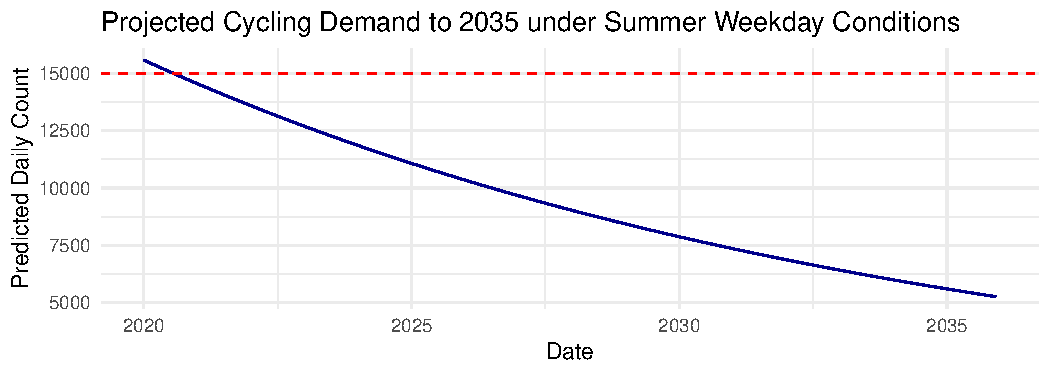
\includegraphics[keepaspectratio,alt={\label{fig:fig-extrapolation}Extrapolation of Cycling Demand}]{Report_project02-1----3000_files/figure-latex/fig-extrapolation-1.pdf}}
\caption{\label{fig:fig-extrapolation}Extrapolation of Cycling Demand}
\end{figure}

\begin{table}[!h]
\centering
\caption{\label{tab:tab-threshold}Earliest projected date at which predicted summer weekday demand exceeds 15,000 cyclists/day.}
\centering
\begin{tabular}[t]{lr}
\toprule
date & pred\_count\\
\midrule
2020-01-01 & 15578.52\\
\bottomrule
\end{tabular}
\end{table}

The extrapolation based on M3 projects decline in Figure \ref{fig:fig-extrapolation}, rather than an increase, summer weekday cycling demand through to 2035. Using the fitted model we can see that the predicted demand is already above the 15,000 cyclists/day threshold at the start of the period, starting at an estimated value of 15,579 on 1 January 2020 as seen in Table \ref{tab:tab-threshold}. It then falls steadily, where in 15 years, the estimated value for cyclists/day is 5,300. This means that, at the current fitted rate, the model does not predict future growth toward the threshold; instead, it suggests that demand moves away from it over time.

This kind of long-run extrapolation should be treated with caution for at least two reasons. First, the fitted linear trend is estimated over a short period, specifically the COVID-19 disruption, where many were forced to stay indoors, hence it may not represent the true long-term path of cycling demand. Secondly, the projection holds weather and seasonal conditions fixed and ignores other factors that could substantially alter future demand. Notably as infrastructure investment, policy changes, fuel prices, or changes in population and commuting patterns. For these reasons, the extrapolation is useful as a simple model-based scenario, but not as a reliable long-term forecast.

\subsubsection{Identifying a poorly-fit period}\label{identifying-a-poorly-fit-period}

This subsection examines the residuals of the final model over time in order to identify a specific period in which the model performs notably poorly. The aim is to determine whether the model systematically over- or under-predicts during that period, and to consider what that implies from both a statistical and transport-planning perspective.

\begin{figure}
\centering
\pandocbounded{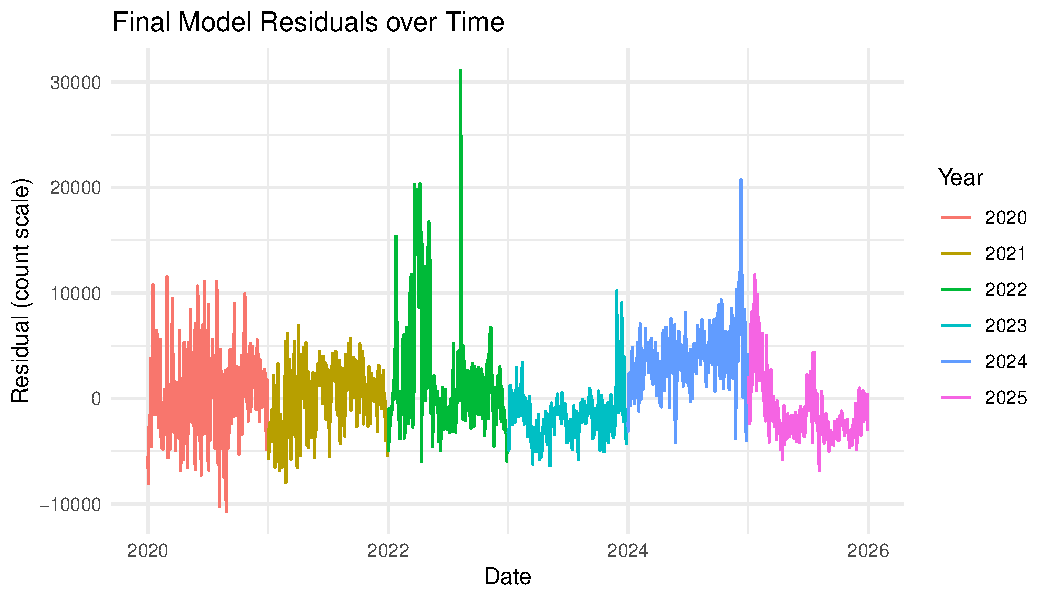
\includegraphics[keepaspectratio,alt={\label{fig:fig-restime}Residuals over Time}]{Report_project02-1----3000_files/figure-latex/fig-restime-1.pdf}}
\caption{\label{fig:fig-restime}Residuals over Time}
\end{figure}

Figure \ref{fig:fig-restime} identifies periods where the final model appears to fit particularly poorly. This can be caused either by residuals that are unusually large in magnitude or because they are persistently positive or negative over a sustained interval.

\begin{table}[!h]
\centering
\caption{\label{tab:tab-poorperiod}Months with the largest RMSE under the final model.}
\centering
\begin{tabular}[t]{lrr}
\toprule
year\_month & mean\_residual & RMSE\\
\midrule
2022-04 & 8934.418 & 11317.815\\
2022-03 & 6851.281 & 10416.665\\
2024-12 & 6009.515 & 7866.465\\
2022-08 & 3602.210 & 7861.138\\
2022-05 & 4191.181 & 7662.392\\
\addlinespace
2024-10 & 5446.711 & 5885.668\\
2025-01 & 4548.762 & 5858.492\\
2022-01 & 1747.584 & 5774.558\\
2024-11 & 4927.126 & 5598.794\\
2024-09 & 4922.280 & 5233.538\\
\bottomrule
\end{tabular}
\end{table}

Table 8 shows the months in which the final model performs worst, ranked by period-specific RMSE. This table will therefore help indicate the exact month with worst performance.

From Table \ref{tab:tab-poorperiod}, we find that April 2022 stands out as the single poorest-fitted month. It has the largest month-specific RMSE in the table, equal to 11317.8, and a positive mean residual of 8934.4. This indicates that the model under-predicts cyclist demand consistently during this period of time rather than making a few isolated large errors.

This implies April 2022 was a period of unusually high cycling demand that is not fully explained by the variables included in the model. The residual plot shows a large grouping of positive residuals during spring and summer 2022. This suggests that the model may be missing some factor that lifted counts above their usual seasonal level.

From a transport-planning perspective, this reflect changes in travel behavior, especially if cycling demand temporarily increased because of favorable or unfavorable conditions. There was potentially a post-pandemic behavioural shifts, where increased free movement was taken advantage. On the other hand, there may have been external factors such as fuel prices. The Ukraine-Russia war started in Feb.2022 and had resulted in significant increases in the prices of crude oil. Statistically, the poor fit also reflects model limitations: the final model includes temperature, seasonality, day of week, and trend, but omits potentially important short-term drivers such as rainfall, wind, holidays, oil prices and special events. April 2022 therefore appears to be a period where both the data limitations and the model specification contribute to poor predictive performance.

\textbf{5.5 Original Diagnostic Plot}

This subsection presents an original plot that is not a standard diagnostic, designed to reveal an interesting feature of the final model that is not visible from standard diagnostics plots. This plot tracks the monthly mean residual over time, showing whether the model systematically over- or under-predicts demand in different periods

\begin{figure}
\centering
\pandocbounded{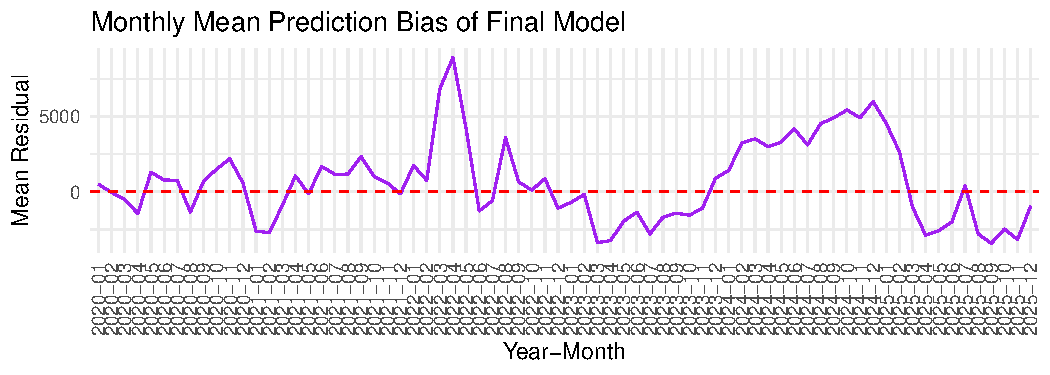
\includegraphics[keepaspectratio,alt={\label{fig:fig-predictionbias}Monthly Mean Prediction Bias}]{Report_project02-1----3000_files/figure-latex/fig-predictionbias-1.pdf}}
\caption{\label{fig:fig-predictionbias}Monthly Mean Prediction Bias}
\end{figure}

The plot in Figure \ref{fig:fig-predictionbias} shows the monthly mean residual of the final model over time. Positive values indicate systematic under-prediction and negative values indicate systematic over-prediction. Multiple periods are visibly out, particularly parts of 2022 and late 2024, where the model persistently under-predicts cycling demand, while much of 2025 shows negative mean residuals, indicating over-prediction. A transport planner should conclude that the model captures overall demand patterns reasonably well, but it struggles to track shifts in underlying behaviour across time. In particular, some periods appear to involve sustained changes in demand that are not fully explained by temperature, seasonality, day of week, and trend alone.

This plot is useful because it highlights regional bias rather than just overall error magnitude. Unlike RMSE or QQ plots, it shows when the model is persistently wrong in one direction, which is especially important for planning. A model that repeatedly under-predicts demand during certain periods may lead planners to underestimate pressure on cycling infrastructure, while persistent over-prediction could lead to over-allocation of resources.

\section{Discussion and limitations}\label{discussion-and-limitations}

Of the four models fitted, M3 comes closest to satisfying the standard linear regression assumptions, though none fully does. M0 through M2 all show indications of heteroscedasticity and a heavy right tail in the QQ plot, which are unsurprising given that daily cyclist counts are non-negative and right-skewed
by nature. The log transformation in M3 largely addresses both problems --- residuals are much more evenly spread and the QQ plot follows the reference line well across most of its range --- but some deviation remains at both tails, so the Gaussian assumption should still be interpreted with some caution even for M3.

The main limitation of the data is that it only includes temperature and calendar variables. Rainfall and wind in particular are likely to affect whether people choose to cycle on a given day, yet neither is available in the dataset. This probably explains why the model struggles most in March and April, and why it consistently under-predicted demand during spring and summer 2022 --- periods where something beyond temperature and seasonality was clearly
driving behaviour. A separate issue is that the response variable pools counts across all monitoring stations, so the model cannot distinguish between commuter routes and leisure routes, which likely behave quite differently.

The long-term trend is also harder to interpret than it first appears. Fitting a single linear trend across 2020--2025 forces the model to average over the COVID dip, the recovery period, and the later years all at once. As the COVID indicator comparison in Section 5.3 shows, this matters --- the trend estimate shifts noticeably depending on how the pandemic period is treated, so the negative trend should not be read as straightforward evidence that cycling in Edinburgh is in structural decline.

The most practical improvements would be to add precipitation and wind speed as predictors, and to replace the linear trend with something more flexible such as a piecewise specification that separates the pandemic period from the rest. A Poisson or negative binomial model would also be a more natural fit for count data and would avoid the back-transformation issue that inflates the DS and IS scores for M3. Longer term, disaggregating to individual monitoring
stations would allow more targeted conclusions about specific routes and corridors.

Finally, it is worth being cautious about how far these findings extend beyond Edinburgh. The temperature effects, commuter patterns, and trend estimate reflect a specific city during an unusual five-year period. A city with a warmer climate or a different cycling culture might show very different seasonal patterns and temperature sensitivity. Even for Edinburgh, the short observation window means the trend extrapolation to 2035 should be treated as an illustrative scenario rather than a forecast --- particularly given how much
the pandemic distorts the earlier part of the data.

\section{Appendix: Code}\label{appendix-code}

All analysis code is in \texttt{code.R} and is reproduced below.

\begin{Shaded}
\begin{Highlighting}[]
\CommentTok{\# ============================================================}
\CommentTok{\# Project 2: Modelling daily cycling demand in Edinburgh}
\CommentTok{\# Authors: [Karthik Sutheeshkumar], [Kiet Lam], [Leon Godtfredsen]}
\CommentTok{\# ============================================================}

\CommentTok{\#}
\CommentTok{\# Place the code needed in the Report\_project02.Rmd, including documentation.}
\CommentTok{\#}

\CommentTok{\# 0. Packages}
\FunctionTok{library}\NormalTok{(ggplot2); }\FunctionTok{library}\NormalTok{(dplyr); }\FunctionTok{library}\NormalTok{(tidyr)}
\FunctionTok{library}\NormalTok{(lubridate); }\FunctionTok{library}\NormalTok{(knitr); }\FunctionTok{library}\NormalTok{(kableExtra)}
\FunctionTok{library}\NormalTok{(patchwork); }\FunctionTok{library}\NormalTok{(broom)}

\CommentTok{\# 1. Load data}
\FunctionTok{load}\NormalTok{(}\StringTok{\textquotesingle{}cycle\_daily\_df.Rdata\textquotesingle{}}\NormalTok{)}

\CommentTok{\# 2. Data Wrangling }
\NormalTok{cycle\_daily\_df }\OtherTok{\textless{}{-}}\NormalTok{ cycle\_daily\_df }\SpecialCharTok{\%\textgreater{}\%}
  \FunctionTok{mutate}\NormalTok{(}
    \AttributeTok{month\_num =}\NormalTok{ month,}
    \AttributeTok{month =} \FunctionTok{factor}\NormalTok{(month, }\AttributeTok{levels =} \DecValTok{1}\SpecialCharTok{:}\DecValTok{12}\NormalTok{, }\AttributeTok{ordered =} \ConstantTok{TRUE}\NormalTok{),}
    \AttributeTok{dow =} \FunctionTok{factor}\NormalTok{(dow, }\AttributeTok{levels =} \FunctionTok{c}\NormalTok{(}\StringTok{"Sun"}\NormalTok{, }\StringTok{"Mon"}\NormalTok{, }\StringTok{"Tue"}\NormalTok{, }\StringTok{"Wed"}\NormalTok{, }\StringTok{"Thu"}\NormalTok{, }\StringTok{"Fri"}\NormalTok{, }\StringTok{"Sat"}\NormalTok{),}
                 \AttributeTok{ordered =} \ConstantTok{TRUE}\NormalTok{),}
    \AttributeTok{trend =} \FunctionTok{as.integer}\NormalTok{(date }\SpecialCharTok{{-}} \FunctionTok{as.Date}\NormalTok{(}\StringTok{"2020{-}01{-}01"}\NormalTok{)),}
    \CommentTok{\#is\_covid = ifelse(year \%in\% 2020:2021, "COVID Period", "Post{-}COVID")}
    
\NormalTok{  )}

\NormalTok{cycle\_cv\_df }\OtherTok{\textless{}{-}}\NormalTok{ cycle\_daily\_df }\SpecialCharTok{\%\textgreater{}\%}
  \FunctionTok{mutate}\NormalTok{(}\AttributeTok{month =} \FunctionTok{as.numeric}\NormalTok{(month))}

\CommentTok{\# 3. Model Fitting}
\CommentTok{\# Note: Use factor(month) in formulas for M1{-}M3}
\NormalTok{model\_formulas }\OtherTok{\textless{}{-}} \FunctionTok{list}\NormalTok{(}
  \AttributeTok{M0 =}\NormalTok{ count }\SpecialCharTok{\textasciitilde{}}\NormalTok{ temp\_mean }\SpecialCharTok{+}\NormalTok{ weekend }\SpecialCharTok{+}\NormalTok{ month\_num,}
  \AttributeTok{M1 =}\NormalTok{ count }\SpecialCharTok{\textasciitilde{}}\NormalTok{ temp\_mean }\SpecialCharTok{+}\NormalTok{ weekend }\SpecialCharTok{+}\NormalTok{ trend }\SpecialCharTok{+} \FunctionTok{factor}\NormalTok{(month) }\SpecialCharTok{+} \FunctionTok{factor}\NormalTok{(dow),}
  \AttributeTok{M2 =}\NormalTok{ count }\SpecialCharTok{\textasciitilde{}}\NormalTok{ weekend }\SpecialCharTok{+}\NormalTok{ trend }\SpecialCharTok{+} \FunctionTok{factor}\NormalTok{(month) }\SpecialCharTok{+} \FunctionTok{factor}\NormalTok{(dow) }\SpecialCharTok{+}
\NormalTok{    temp\_mean }\SpecialCharTok{+} \FunctionTok{I}\NormalTok{(temp\_mean}\SpecialCharTok{\^{}}\DecValTok{2}\NormalTok{),}
  \AttributeTok{M3 =} \FunctionTok{log}\NormalTok{(count }\SpecialCharTok{+} \DecValTok{1}\NormalTok{) }\SpecialCharTok{\textasciitilde{}}\NormalTok{ weekend }\SpecialCharTok{+}\NormalTok{ trend }\SpecialCharTok{+} \FunctionTok{factor}\NormalTok{(month) }\SpecialCharTok{+} \FunctionTok{factor}\NormalTok{(dow) }\SpecialCharTok{+}
\NormalTok{    temp\_mean }\SpecialCharTok{+} \FunctionTok{I}\NormalTok{(temp\_mean}\SpecialCharTok{\^{}}\DecValTok{2}\NormalTok{) }\CommentTok{\#+ is\_covid}
\NormalTok{)}

\NormalTok{m0 }\OtherTok{\textless{}{-}} \FunctionTok{lm}\NormalTok{(model\_formulas[[}\StringTok{"M0"}\NormalTok{]], }\AttributeTok{data =}\NormalTok{ cycle\_daily\_df)}
\NormalTok{m1 }\OtherTok{\textless{}{-}} \FunctionTok{lm}\NormalTok{(model\_formulas[[}\StringTok{"M1"}\NormalTok{]], }\AttributeTok{data =}\NormalTok{ cycle\_daily\_df)}
\NormalTok{m2 }\OtherTok{\textless{}{-}} \FunctionTok{lm}\NormalTok{(model\_formulas[[}\StringTok{"M2"}\NormalTok{]], }\AttributeTok{data =}\NormalTok{ cycle\_daily\_df)}
\NormalTok{m3 }\OtherTok{\textless{}{-}} \FunctionTok{lm}\NormalTok{(model\_formulas[[}\StringTok{"M3"}\NormalTok{]], }\AttributeTok{data =}\NormalTok{ cycle\_daily\_df)}

\CommentTok{\# 4. Cross{-}Validation Functions}
\NormalTok{calc\_scores }\OtherTok{\textless{}{-}} \ControlFlowTok{function}\NormalTok{(y, mu, sigma, }\AttributeTok{alpha =} \FloatTok{0.05}\NormalTok{) \{}
  \CommentTok{\# y     : vector of observed values}
  \CommentTok{\# mu    : vector of predictive means (from predict(fit, newdata=test)$fit)}
  \CommentTok{\# sigma : vector of predictive SDs. Combine residual error and mean uncertainty:}
  \CommentTok{\#         sigma = sqrt(summary(fit)$sigma\^{}2 + predict(fit, newdata=test, se.fit=TRUE)$se.fit\^{}2)}
  \CommentTok{\# Returns a named list with RMSE, MAE, DS, IS}
  
  \CommentTok{\# Implement RMSE, MAE, DS, and IS here}
  
\NormalTok{  RMSE }\OtherTok{\textless{}{-}} \FunctionTok{sqrt}\NormalTok{(}\FunctionTok{mean}\NormalTok{((y}\SpecialCharTok{{-}}\NormalTok{mu)}\SpecialCharTok{\^{}}\DecValTok{2}\NormalTok{))}
\NormalTok{  MAE }\OtherTok{\textless{}{-}} \FunctionTok{mean}\NormalTok{(}\FunctionTok{abs}\NormalTok{(y}\SpecialCharTok{{-}}\NormalTok{mu))}
\NormalTok{  DS }\OtherTok{\textless{}{-}}\NormalTok{ (y}\SpecialCharTok{{-}}\NormalTok{mu)}\SpecialCharTok{\^{}}\DecValTok{2}\SpecialCharTok{/}\NormalTok{sigma}\SpecialCharTok{\^{}}\DecValTok{2} \SpecialCharTok{+} \DecValTok{2} \SpecialCharTok{*} \FunctionTok{log}\NormalTok{(sigma)}
\NormalTok{  l  }\OtherTok{\textless{}{-}}\NormalTok{ mu }\SpecialCharTok{{-}} \FunctionTok{qnorm}\NormalTok{(}\DecValTok{1} \SpecialCharTok{{-}}\NormalTok{ alpha}\SpecialCharTok{/}\DecValTok{2}\NormalTok{) }\SpecialCharTok{*}\NormalTok{ sigma}
\NormalTok{  u  }\OtherTok{\textless{}{-}}\NormalTok{ mu }\SpecialCharTok{+} \FunctionTok{qnorm}\NormalTok{(}\DecValTok{1} \SpecialCharTok{{-}}\NormalTok{ alpha}\SpecialCharTok{/}\DecValTok{2}\NormalTok{) }\SpecialCharTok{*}\NormalTok{ sigma}
\NormalTok{  IS }\OtherTok{\textless{}{-}}\NormalTok{ (u}\SpecialCharTok{{-}}\NormalTok{l) }\SpecialCharTok{+}\NormalTok{ (}\DecValTok{2}\SpecialCharTok{/}\NormalTok{alpha)}\SpecialCharTok{*}\FunctionTok{pmax}\NormalTok{(l}\SpecialCharTok{{-}}\NormalTok{y,}\DecValTok{0}\NormalTok{) }\SpecialCharTok{+}\NormalTok{ (}\DecValTok{2}\SpecialCharTok{/}\NormalTok{alpha)}\SpecialCharTok{*}\FunctionTok{pmax}\NormalTok{(y}\SpecialCharTok{{-}}\NormalTok{u,}\DecValTok{0}\NormalTok{)}
  \FunctionTok{return}\NormalTok{(}\FunctionTok{list}\NormalTok{(}\AttributeTok{RMSE =}\NormalTok{ RMSE, }\AttributeTok{MAE =}\NormalTok{ MAE, }\AttributeTok{DS =}\NormalTok{ DS, }\AttributeTok{IS =}\NormalTok{ IS))}

\NormalTok{\}}

\CommentTok{\# 5. Leave{-}One{-}Year{-}Out CV Loop }
\NormalTok{years }\OtherTok{\textless{}{-}}\FunctionTok{unique}\NormalTok{(cycle\_cv\_df}\SpecialCharTok{$}\NormalTok{year)}

\NormalTok{cv\_results }\OtherTok{\textless{}{-}} \FunctionTok{bind\_rows}\NormalTok{(}\FunctionTok{lapply}\NormalTok{(}\FunctionTok{names}\NormalTok{(model\_formulas), }\ControlFlowTok{function}\NormalTok{(model\_name) \{}
  \FunctionTok{bind\_rows}\NormalTok{(}\FunctionTok{lapply}\NormalTok{(years, }\ControlFlowTok{function}\NormalTok{(yr) \{}
    
    \CommentTok{\# Splitting into train and test}
\NormalTok{    test\_df  }\OtherTok{\textless{}{-}}\NormalTok{ cycle\_cv\_df }\SpecialCharTok{\%\textgreater{}\%} \FunctionTok{filter}\NormalTok{(year }\SpecialCharTok{==}\NormalTok{ yr)}
\NormalTok{    train\_df }\OtherTok{\textless{}{-}}\NormalTok{ cycle\_cv\_df }\SpecialCharTok{\%\textgreater{}\%} \FunctionTok{filter}\NormalTok{(year }\SpecialCharTok{!=}\NormalTok{ yr)}
    
    \CommentTok{\# Fitting model on training data }
\NormalTok{    fit }\OtherTok{\textless{}{-}} \FunctionTok{lm}\NormalTok{(model\_formulas[[model\_name]], }\AttributeTok{data =}\NormalTok{ train\_df)}
    
    \CommentTok{\# Predicting on test data}
\NormalTok{    pred  }\OtherTok{\textless{}{-}} \FunctionTok{predict}\NormalTok{(fit, }\AttributeTok{newdata =}\NormalTok{ test\_df, }\AttributeTok{se.fit =} \ConstantTok{TRUE}\NormalTok{)}
\NormalTok{    mu    }\OtherTok{\textless{}{-}}\NormalTok{ pred}\SpecialCharTok{$}\NormalTok{fit}
\NormalTok{    sigma }\OtherTok{\textless{}{-}} \FunctionTok{sqrt}\NormalTok{(}\FunctionTok{summary}\NormalTok{(fit)}\SpecialCharTok{$}\NormalTok{sigma}\SpecialCharTok{\^{}}\DecValTok{2} \SpecialCharTok{+}\NormalTok{ pred}\SpecialCharTok{$}\NormalTok{se.fit}\SpecialCharTok{\^{}}\DecValTok{2}\NormalTok{)}
    
    \CommentTok{\# Observed values from test\_df}
\NormalTok{    y }\OtherTok{\textless{}{-}}\NormalTok{ test\_df}\SpecialCharTok{$}\NormalTok{count}
    
    \CommentTok{\# Case for M3 }
    \ControlFlowTok{if}\NormalTok{ (model\_name }\SpecialCharTok{==} \StringTok{"M3"}\NormalTok{) \{}
\NormalTok{      mu\_log    }\OtherTok{\textless{}{-}}\NormalTok{ mu}
\NormalTok{      sigma\_log }\OtherTok{\textless{}{-}}\NormalTok{ sigma}
      
      \CommentTok{\# Back{-}transform to count scale}
\NormalTok{      mu\_count    }\OtherTok{\textless{}{-}} \FunctionTok{exp}\NormalTok{(mu\_log) }\SpecialCharTok{{-}} \DecValTok{1}
\NormalTok{      sigma\_count }\OtherTok{\textless{}{-}} \FunctionTok{exp}\NormalTok{(mu\_log) }\SpecialCharTok{*}\NormalTok{ sigma\_log  }\CommentTok{\# delta method}
      \CommentTok{\#sigma\_count \textless{}{-} sqrt((exp(sigma\_log\^{}2) {-} 1) * exp(2 * mu\_log + sigma\_log\^{}2))}
      
\NormalTok{      y }\OtherTok{\textless{}{-}}\NormalTok{ test\_df}\SpecialCharTok{$}\NormalTok{count}
      
\NormalTok{      CV\_scores }\OtherTok{\textless{}{-}} \FunctionTok{calc\_scores}\NormalTok{(y, mu\_count, sigma\_count)}
      
      \FunctionTok{return}\NormalTok{(}\FunctionTok{data.frame}\NormalTok{(}
        \AttributeTok{model =}\NormalTok{ model\_name,}
        \AttributeTok{year  =}\NormalTok{ yr,}
        \AttributeTok{RMSE  =}\NormalTok{ CV\_scores}\SpecialCharTok{$}\NormalTok{RMSE,}
        \AttributeTok{MAE   =}\NormalTok{ CV\_scores}\SpecialCharTok{$}\NormalTok{MAE,}
        \AttributeTok{DS    =} \FunctionTok{mean}\NormalTok{(CV\_scores}\SpecialCharTok{$}\NormalTok{DS),}
        \AttributeTok{IS    =} \FunctionTok{mean}\NormalTok{(CV\_scores}\SpecialCharTok{$}\NormalTok{IS)}
\NormalTok{      ))}
\NormalTok{    \}}
    \CommentTok{\# CV score predictions against observed values}
\NormalTok{    CV\_scores }\OtherTok{\textless{}{-}} \FunctionTok{calc\_scores}\NormalTok{(y, mu, sigma)}
    
    \FunctionTok{data.frame}\NormalTok{(}
      \AttributeTok{model =}\NormalTok{ model\_name,}
      \AttributeTok{year  =}\NormalTok{ yr,}
      \AttributeTok{RMSE  =}\NormalTok{ CV\_scores}\SpecialCharTok{$}\NormalTok{RMSE,}
      \AttributeTok{MAE   =}\NormalTok{ CV\_scores}\SpecialCharTok{$}\NormalTok{MAE,}
      \AttributeTok{DS    =} \FunctionTok{mean}\NormalTok{(CV\_scores}\SpecialCharTok{$}\NormalTok{DS),}
      \AttributeTok{IS    =} \FunctionTok{mean}\NormalTok{(CV\_scores}\SpecialCharTok{$}\NormalTok{IS)}
\NormalTok{    )}
\NormalTok{  \}))}
\NormalTok{\}))}

\CommentTok{\# Table 1: average scores across all held{-}out years}
\NormalTok{cv\_table1 }\OtherTok{\textless{}{-}}\NormalTok{ cv\_results }\SpecialCharTok{\%\textgreater{}\%}
  \FunctionTok{group\_by}\NormalTok{(model) }\SpecialCharTok{\%\textgreater{}\%}
  \FunctionTok{summarise}\NormalTok{(}
    \AttributeTok{RMSE =} \FunctionTok{round}\NormalTok{(}\FunctionTok{mean}\NormalTok{(RMSE), }\DecValTok{1}\NormalTok{),}
    \AttributeTok{MAE  =} \FunctionTok{round}\NormalTok{(}\FunctionTok{mean}\NormalTok{(MAE), }\DecValTok{1}\NormalTok{),}
    \AttributeTok{DS   =} \FunctionTok{round}\NormalTok{(}\FunctionTok{mean}\NormalTok{(DS), }\DecValTok{2}\NormalTok{),}
    \AttributeTok{IS   =} \FunctionTok{round}\NormalTok{(}\FunctionTok{mean}\NormalTok{(IS),}\DecValTok{1}\NormalTok{),}
    \AttributeTok{.groups =} \StringTok{"drop"}
\NormalTok{  )}

\FunctionTok{print}\NormalTok{(cv\_table1)}


\CommentTok{\# 6. CV by Month }

\CommentTok{\# Create an empty data frame to store observation{-}level CV predictions}
\NormalTok{cv\_month\_data }\OtherTok{\textless{}{-}}\NormalTok{ cycle\_cv\_df }\SpecialCharTok{\%\textgreater{}\%}
  \FunctionTok{mutate}\NormalTok{(}
    \AttributeTok{mean\_M0 =} \ConstantTok{NA\_real\_}\NormalTok{, }\AttributeTok{sd\_M0 =} \ConstantTok{NA\_real\_}\NormalTok{,}
    \AttributeTok{mean\_M1 =} \ConstantTok{NA\_real\_}\NormalTok{, }\AttributeTok{sd\_M1 =} \ConstantTok{NA\_real\_}\NormalTok{,}
    \AttributeTok{mean\_M2 =} \ConstantTok{NA\_real\_}\NormalTok{, }\AttributeTok{sd\_M2 =} \ConstantTok{NA\_real\_}\NormalTok{,}
    \AttributeTok{mean\_M3 =} \ConstantTok{NA\_real\_}\NormalTok{, }\AttributeTok{sd\_M3 =} \ConstantTok{NA\_real\_}
\NormalTok{  )}

\CommentTok{\# Fill in leave{-}one{-}year{-}out predictions for each model}
\ControlFlowTok{for}\NormalTok{ (yr }\ControlFlowTok{in}\NormalTok{ years) \{}
  
\NormalTok{  train\_data }\OtherTok{\textless{}{-}}\NormalTok{ cycle\_cv\_df }\SpecialCharTok{\%\textgreater{}\%} \FunctionTok{filter}\NormalTok{(year }\SpecialCharTok{!=}\NormalTok{ yr)}
\NormalTok{  test\_ind   }\OtherTok{\textless{}{-}} \FunctionTok{which}\NormalTok{(cycle\_cv\_df}\SpecialCharTok{$}\NormalTok{year }\SpecialCharTok{==}\NormalTok{ yr)}
\NormalTok{  test\_data  }\OtherTok{\textless{}{-}}\NormalTok{ cycle\_cv\_df[test\_ind, , drop }\OtherTok{=} \ConstantTok{FALSE}\NormalTok{]}
  
  \CommentTok{\# M0}
\NormalTok{  fit\_M0 }\OtherTok{\textless{}{-}} \FunctionTok{lm}\NormalTok{(model\_formulas[[}\StringTok{"M0"}\NormalTok{]], }\AttributeTok{data =}\NormalTok{ train\_data)}
\NormalTok{  pred\_M0 }\OtherTok{\textless{}{-}} \FunctionTok{predict}\NormalTok{(fit\_M0, }\AttributeTok{newdata =}\NormalTok{ test\_data, }\AttributeTok{se.fit =} \ConstantTok{TRUE}\NormalTok{)}
\NormalTok{  cv\_month\_data[test\_ind, }\StringTok{"mean\_M0"}\NormalTok{] }\OtherTok{\textless{}{-}}\NormalTok{ pred\_M0}\SpecialCharTok{$}\NormalTok{fit}
\NormalTok{  cv\_month\_data[test\_ind, }\StringTok{"sd\_M0"}\NormalTok{] }\OtherTok{\textless{}{-}} \FunctionTok{sqrt}\NormalTok{(pred\_M0}\SpecialCharTok{$}\NormalTok{se.fit}\SpecialCharTok{\^{}}\DecValTok{2} \SpecialCharTok{+} \FunctionTok{summary}\NormalTok{(fit\_M0)}\SpecialCharTok{$}\NormalTok{sigma}\SpecialCharTok{\^{}}\DecValTok{2}\NormalTok{)}
  
  \CommentTok{\# M1}
\NormalTok{  fit\_M1 }\OtherTok{\textless{}{-}} \FunctionTok{lm}\NormalTok{(model\_formulas[[}\StringTok{"M1"}\NormalTok{]], }\AttributeTok{data =}\NormalTok{ train\_data)}
\NormalTok{  pred\_M1 }\OtherTok{\textless{}{-}} \FunctionTok{predict}\NormalTok{(fit\_M1, }\AttributeTok{newdata =}\NormalTok{ test\_data, }\AttributeTok{se.fit =} \ConstantTok{TRUE}\NormalTok{)}
\NormalTok{  cv\_month\_data[test\_ind, }\StringTok{"mean\_M1"}\NormalTok{] }\OtherTok{\textless{}{-}}\NormalTok{ pred\_M1}\SpecialCharTok{$}\NormalTok{fit}
\NormalTok{  cv\_month\_data[test\_ind, }\StringTok{"sd\_M1"}\NormalTok{] }\OtherTok{\textless{}{-}} \FunctionTok{sqrt}\NormalTok{(pred\_M1}\SpecialCharTok{$}\NormalTok{se.fit}\SpecialCharTok{\^{}}\DecValTok{2} \SpecialCharTok{+} \FunctionTok{summary}\NormalTok{(fit\_M1)}\SpecialCharTok{$}\NormalTok{sigma}\SpecialCharTok{\^{}}\DecValTok{2}\NormalTok{)}
  
  \CommentTok{\# M2}
\NormalTok{  fit\_M2 }\OtherTok{\textless{}{-}} \FunctionTok{lm}\NormalTok{(model\_formulas[[}\StringTok{"M2"}\NormalTok{]], }\AttributeTok{data =}\NormalTok{ train\_data)}
\NormalTok{  pred\_M2 }\OtherTok{\textless{}{-}} \FunctionTok{predict}\NormalTok{(fit\_M2, }\AttributeTok{newdata =}\NormalTok{ test\_data, }\AttributeTok{se.fit =} \ConstantTok{TRUE}\NormalTok{)}
\NormalTok{  cv\_month\_data[test\_ind, }\StringTok{"mean\_M2"}\NormalTok{] }\OtherTok{\textless{}{-}}\NormalTok{ pred\_M2}\SpecialCharTok{$}\NormalTok{fit}
\NormalTok{  cv\_month\_data[test\_ind, }\StringTok{"sd\_M2"}\NormalTok{] }\OtherTok{\textless{}{-}} \FunctionTok{sqrt}\NormalTok{(pred\_M2}\SpecialCharTok{$}\NormalTok{se.fit}\SpecialCharTok{\^{}}\DecValTok{2} \SpecialCharTok{+} \FunctionTok{summary}\NormalTok{(fit\_M2)}\SpecialCharTok{$}\NormalTok{sigma}\SpecialCharTok{\^{}}\DecValTok{2}\NormalTok{)}
  
  \CommentTok{\# M3}
\NormalTok{  fit\_M3 }\OtherTok{\textless{}{-}} \FunctionTok{lm}\NormalTok{(model\_formulas[[}\StringTok{"M3"}\NormalTok{]], }\AttributeTok{data =}\NormalTok{ train\_data)}
\NormalTok{  pred\_M3 }\OtherTok{\textless{}{-}} \FunctionTok{predict}\NormalTok{(fit\_M3, }\AttributeTok{newdata =}\NormalTok{ test\_data, }\AttributeTok{se.fit =} \ConstantTok{TRUE}\NormalTok{)}
\NormalTok{  cv\_month\_data[test\_ind, }\StringTok{"mean\_M3"}\NormalTok{] }\OtherTok{\textless{}{-}}\NormalTok{ pred\_M3}\SpecialCharTok{$}\NormalTok{fit}
\NormalTok{  cv\_month\_data[test\_ind, }\StringTok{"sd\_M3"}\NormalTok{] }\OtherTok{\textless{}{-}} \FunctionTok{sqrt}\NormalTok{(pred\_M3}\SpecialCharTok{$}\NormalTok{se.fit}\SpecialCharTok{\^{}}\DecValTok{2} \SpecialCharTok{+} \FunctionTok{summary}\NormalTok{(fit\_M3)}\SpecialCharTok{$}\NormalTok{sigma}\SpecialCharTok{\^{}}\DecValTok{2}\NormalTok{)}
\NormalTok{\}}

\CommentTok{\# Compute scores for each observation}
\NormalTok{score\_month }\OtherTok{\textless{}{-}}\NormalTok{ cv\_month\_data }\SpecialCharTok{\%\textgreater{}\%}
  \FunctionTok{mutate}\NormalTok{(}
    \AttributeTok{se\_M0 =}\NormalTok{ (count }\SpecialCharTok{{-}}\NormalTok{ mean\_M0)}\SpecialCharTok{\^{}}\DecValTok{2}\NormalTok{,}
    \AttributeTok{ds\_M0 =}\NormalTok{ (count }\SpecialCharTok{{-}}\NormalTok{ mean\_M0)}\SpecialCharTok{\^{}}\DecValTok{2} \SpecialCharTok{/}\NormalTok{ sd\_M0}\SpecialCharTok{\^{}}\DecValTok{2} \SpecialCharTok{+} \DecValTok{2} \SpecialCharTok{*} \FunctionTok{log}\NormalTok{(sd\_M0),}
    \AttributeTok{lwr\_M0 =}\NormalTok{ mean\_M0 }\SpecialCharTok{{-}} \FunctionTok{qnorm}\NormalTok{(}\FloatTok{0.975}\NormalTok{) }\SpecialCharTok{*}\NormalTok{ sd\_M0,}
    \AttributeTok{upr\_M0 =}\NormalTok{ mean\_M0 }\SpecialCharTok{+} \FunctionTok{qnorm}\NormalTok{(}\FloatTok{0.975}\NormalTok{) }\SpecialCharTok{*}\NormalTok{ sd\_M0,}
    \AttributeTok{is\_M0 =}\NormalTok{ (upr\_M0 }\SpecialCharTok{{-}}\NormalTok{ lwr\_M0) }\SpecialCharTok{+}
\NormalTok{      (}\DecValTok{2} \SpecialCharTok{/} \FloatTok{0.05}\NormalTok{) }\SpecialCharTok{*} \FunctionTok{pmax}\NormalTok{(lwr\_M0 }\SpecialCharTok{{-}}\NormalTok{ count, }\DecValTok{0}\NormalTok{) }\SpecialCharTok{+}
\NormalTok{      (}\DecValTok{2} \SpecialCharTok{/} \FloatTok{0.05}\NormalTok{) }\SpecialCharTok{*} \FunctionTok{pmax}\NormalTok{(count }\SpecialCharTok{{-}}\NormalTok{ upr\_M0, }\DecValTok{0}\NormalTok{),}
    
    \AttributeTok{se\_M1 =}\NormalTok{ (count }\SpecialCharTok{{-}}\NormalTok{ mean\_M1)}\SpecialCharTok{\^{}}\DecValTok{2}\NormalTok{,}
    \AttributeTok{ds\_M1 =}\NormalTok{ (count }\SpecialCharTok{{-}}\NormalTok{ mean\_M1)}\SpecialCharTok{\^{}}\DecValTok{2} \SpecialCharTok{/}\NormalTok{ sd\_M1}\SpecialCharTok{\^{}}\DecValTok{2} \SpecialCharTok{+} \DecValTok{2} \SpecialCharTok{*} \FunctionTok{log}\NormalTok{(sd\_M1),}
    \AttributeTok{lwr\_M1 =}\NormalTok{ mean\_M1 }\SpecialCharTok{{-}} \FunctionTok{qnorm}\NormalTok{(}\FloatTok{0.975}\NormalTok{) }\SpecialCharTok{*}\NormalTok{ sd\_M1,}
    \AttributeTok{upr\_M1 =}\NormalTok{ mean\_M1 }\SpecialCharTok{+} \FunctionTok{qnorm}\NormalTok{(}\FloatTok{0.975}\NormalTok{) }\SpecialCharTok{*}\NormalTok{ sd\_M1,}
    \AttributeTok{is\_M1 =}\NormalTok{ (upr\_M1 }\SpecialCharTok{{-}}\NormalTok{ lwr\_M1) }\SpecialCharTok{+}
\NormalTok{      (}\DecValTok{2} \SpecialCharTok{/} \FloatTok{0.05}\NormalTok{) }\SpecialCharTok{*} \FunctionTok{pmax}\NormalTok{(lwr\_M1 }\SpecialCharTok{{-}}\NormalTok{ count, }\DecValTok{0}\NormalTok{) }\SpecialCharTok{+}
\NormalTok{      (}\DecValTok{2} \SpecialCharTok{/} \FloatTok{0.05}\NormalTok{) }\SpecialCharTok{*} \FunctionTok{pmax}\NormalTok{(count }\SpecialCharTok{{-}}\NormalTok{ upr\_M1, }\DecValTok{0}\NormalTok{),}
    
    \AttributeTok{se\_M2 =}\NormalTok{ (count }\SpecialCharTok{{-}}\NormalTok{ mean\_M2)}\SpecialCharTok{\^{}}\DecValTok{2}\NormalTok{,}
    \AttributeTok{ds\_M2 =}\NormalTok{ (count }\SpecialCharTok{{-}}\NormalTok{ mean\_M2)}\SpecialCharTok{\^{}}\DecValTok{2} \SpecialCharTok{/}\NormalTok{ sd\_M2}\SpecialCharTok{\^{}}\DecValTok{2} \SpecialCharTok{+} \DecValTok{2} \SpecialCharTok{*} \FunctionTok{log}\NormalTok{(sd\_M2),}
    \AttributeTok{lwr\_M2 =}\NormalTok{ mean\_M2 }\SpecialCharTok{{-}} \FunctionTok{qnorm}\NormalTok{(}\FloatTok{0.975}\NormalTok{) }\SpecialCharTok{*}\NormalTok{ sd\_M2,}
    \AttributeTok{upr\_M2 =}\NormalTok{ mean\_M2 }\SpecialCharTok{+} \FunctionTok{qnorm}\NormalTok{(}\FloatTok{0.975}\NormalTok{) }\SpecialCharTok{*}\NormalTok{ sd\_M2,}
    \AttributeTok{is\_M2 =}\NormalTok{ (upr\_M2 }\SpecialCharTok{{-}}\NormalTok{ lwr\_M2) }\SpecialCharTok{+}
\NormalTok{      (}\DecValTok{2} \SpecialCharTok{/} \FloatTok{0.05}\NormalTok{) }\SpecialCharTok{*} \FunctionTok{pmax}\NormalTok{(lwr\_M2 }\SpecialCharTok{{-}}\NormalTok{ count, }\DecValTok{0}\NormalTok{) }\SpecialCharTok{+}
\NormalTok{      (}\DecValTok{2} \SpecialCharTok{/} \FloatTok{0.05}\NormalTok{) }\SpecialCharTok{*} \FunctionTok{pmax}\NormalTok{(count }\SpecialCharTok{{-}}\NormalTok{ upr\_M2, }\DecValTok{0}\NormalTok{),}
    
    \AttributeTok{mean\_M3\_count    =} \FunctionTok{exp}\NormalTok{(mean\_M3) }\SpecialCharTok{{-}} \DecValTok{1}\NormalTok{,}
    \AttributeTok{sigma\_count =} \FunctionTok{exp}\NormalTok{(mean\_M3) }\SpecialCharTok{*}\NormalTok{ sd\_M3,}
    
    \AttributeTok{se\_M3  =}\NormalTok{ (count }\SpecialCharTok{{-}}\NormalTok{ mean\_M3\_count)}\SpecialCharTok{\^{}}\DecValTok{2}\NormalTok{,}
    \AttributeTok{ds\_M3  =}\NormalTok{ (count }\SpecialCharTok{{-}}\NormalTok{ mean\_M3\_count)}\SpecialCharTok{\^{}}\DecValTok{2} \SpecialCharTok{/}\NormalTok{ sigma\_count}\SpecialCharTok{\^{}}\DecValTok{2} \SpecialCharTok{+} \DecValTok{2} \SpecialCharTok{*} \FunctionTok{log}\NormalTok{(sigma\_count),}
    
    \AttributeTok{lwr\_M3 =} \FunctionTok{exp}\NormalTok{(mean\_M3 }\SpecialCharTok{{-}} \FunctionTok{qnorm}\NormalTok{(}\FloatTok{0.975}\NormalTok{) }\SpecialCharTok{*}\NormalTok{ sd\_M3) }\SpecialCharTok{{-}} \DecValTok{1}\NormalTok{,}
    \AttributeTok{upr\_M3 =} \FunctionTok{exp}\NormalTok{(mean\_M3 }\SpecialCharTok{+} \FunctionTok{qnorm}\NormalTok{(}\FloatTok{0.975}\NormalTok{) }\SpecialCharTok{*}\NormalTok{ sd\_M3) }\SpecialCharTok{{-}} \DecValTok{1}\NormalTok{,}
    
    \AttributeTok{is\_M3  =}\NormalTok{ (upr\_M3 }\SpecialCharTok{{-}}\NormalTok{ lwr\_M3) }\SpecialCharTok{+}
\NormalTok{      (}\DecValTok{2} \SpecialCharTok{/} \FloatTok{0.05}\NormalTok{) }\SpecialCharTok{*} \FunctionTok{pmax}\NormalTok{(lwr\_M3 }\SpecialCharTok{{-}}\NormalTok{ count, }\DecValTok{0}\NormalTok{) }\SpecialCharTok{+}
\NormalTok{      (}\DecValTok{2} \SpecialCharTok{/} \FloatTok{0.05}\NormalTok{) }\SpecialCharTok{*} \FunctionTok{pmax}\NormalTok{(count }\SpecialCharTok{{-}}\NormalTok{ upr\_M3, }\DecValTok{0}\NormalTok{)}
    
    
    \CommentTok{\#mean\_M3\_count = exp(mean\_M3) {-} 1,}
    \CommentTok{\#se\_M3 = (count {-} mean\_M3\_count)\^{}2,}
    \CommentTok{\#ds\_M3 = (log(count + 1) {-} mean\_M3)\^{}2 / sd\_M3\^{}2 + 2 * log(sd\_M3),}
    \CommentTok{\#mu\_count    = exp(mean\_M3) {-} 1,}
    \CommentTok{\#sigma\_count = exp(mean\_M3) * sd\_M3,}
    \CommentTok{\#ds\_M3 = (count {-} mu\_count)\^{}2 / sigma\_count\^{}2 + 2 * log(sigma\_count),}
    
    \CommentTok{\#lwr\_M3 = exp(mean\_M3 {-} qnorm(0.975) * sd\_M3) {-} 1,}
    \CommentTok{\#upr\_M3 = exp(mean\_M3 + qnorm(0.975) * sd\_M3) {-} 1,}
    
    \CommentTok{\#lwr\_M3 = mean\_M3 {-} qnorm(0.975) * sd\_M3,}
    \CommentTok{\#upr\_M3 = mean\_M3 + qnorm(0.975) * sd\_M3,}
    \CommentTok{\#is\_M3 = (upr\_M3 {-} lwr\_M3) +}
      \CommentTok{\#(2 / 0.05) * pmax(lwr\_M3 {-} log(count + 1), 0) +}
      \CommentTok{\#(2 / 0.05) * pmax(log(count + 1) {-} upr\_M3, 0)}
\NormalTok{  )}

\CommentTok{\# Summarise scores by month}
\NormalTok{cv\_month\_allmodels }\OtherTok{\textless{}{-}}\NormalTok{ score\_month }\SpecialCharTok{\%\textgreater{}\%}
  \FunctionTok{group\_by}\NormalTok{(month) }\SpecialCharTok{\%\textgreater{}\%}
  \FunctionTok{summarise}\NormalTok{(}
    \AttributeTok{RMSE\_M0 =} \FunctionTok{round}\NormalTok{(}\FunctionTok{sqrt}\NormalTok{(}\FunctionTok{mean}\NormalTok{(se\_M0)), }\DecValTok{1}\NormalTok{),}
    \AttributeTok{MAE\_M0  =} \FunctionTok{round}\NormalTok{(}\FunctionTok{mean}\NormalTok{(}\FunctionTok{abs}\NormalTok{(count }\SpecialCharTok{{-}}\NormalTok{ mean\_M0)), }\DecValTok{1}\NormalTok{),}
    \AttributeTok{DS\_M0   =} \FunctionTok{round}\NormalTok{(}\FunctionTok{mean}\NormalTok{(ds\_M0), }\DecValTok{2}\NormalTok{),}
    \AttributeTok{IS\_M0   =} \FunctionTok{round}\NormalTok{(}\FunctionTok{mean}\NormalTok{(is\_M0), }\DecValTok{1}\NormalTok{),}
    
    \AttributeTok{RMSE\_M1 =} \FunctionTok{round}\NormalTok{(}\FunctionTok{sqrt}\NormalTok{(}\FunctionTok{mean}\NormalTok{(se\_M1)), }\DecValTok{1}\NormalTok{),}
    \AttributeTok{MAE\_M1  =} \FunctionTok{round}\NormalTok{(}\FunctionTok{mean}\NormalTok{(}\FunctionTok{abs}\NormalTok{(count }\SpecialCharTok{{-}}\NormalTok{ mean\_M1)), }\DecValTok{1}\NormalTok{),}
    \AttributeTok{DS\_M1   =} \FunctionTok{round}\NormalTok{(}\FunctionTok{mean}\NormalTok{(ds\_M1), }\DecValTok{2}\NormalTok{),}
    \AttributeTok{IS\_M1   =} \FunctionTok{round}\NormalTok{(}\FunctionTok{mean}\NormalTok{(is\_M1), }\DecValTok{1}\NormalTok{),}
    
    \AttributeTok{RMSE\_M2 =} \FunctionTok{round}\NormalTok{(}\FunctionTok{sqrt}\NormalTok{(}\FunctionTok{mean}\NormalTok{(se\_M2)), }\DecValTok{1}\NormalTok{),}
    \AttributeTok{MAE\_M2  =} \FunctionTok{round}\NormalTok{(}\FunctionTok{mean}\NormalTok{(}\FunctionTok{abs}\NormalTok{(count }\SpecialCharTok{{-}}\NormalTok{ mean\_M2)), }\DecValTok{1}\NormalTok{),}
    \AttributeTok{DS\_M2   =} \FunctionTok{round}\NormalTok{(}\FunctionTok{mean}\NormalTok{(ds\_M2), }\DecValTok{2}\NormalTok{),}
    \AttributeTok{IS\_M2   =} \FunctionTok{round}\NormalTok{(}\FunctionTok{mean}\NormalTok{(is\_M2), }\DecValTok{1}\NormalTok{),}
    
    \AttributeTok{RMSE\_M3 =} \FunctionTok{round}\NormalTok{(}\FunctionTok{sqrt}\NormalTok{(}\FunctionTok{mean}\NormalTok{(se\_M3)), }\DecValTok{1}\NormalTok{),}
    \AttributeTok{MAE\_M3  =} \FunctionTok{round}\NormalTok{(}\FunctionTok{mean}\NormalTok{(}\FunctionTok{abs}\NormalTok{(count }\SpecialCharTok{{-}}\NormalTok{ mean\_M3\_count)), }\DecValTok{1}\NormalTok{),}
    \AttributeTok{DS\_M3   =} \FunctionTok{round}\NormalTok{(}\FunctionTok{mean}\NormalTok{(ds\_M3), }\DecValTok{2}\NormalTok{),}
    \AttributeTok{IS\_M3   =} \FunctionTok{round}\NormalTok{(}\FunctionTok{mean}\NormalTok{(is\_M3), }\DecValTok{1}\NormalTok{)}
\NormalTok{  )}

\FunctionTok{print}\NormalTok{(cv\_month\_allmodels)}

\CommentTok{\#Model3 }

\NormalTok{cv\_table2 }\OtherTok{\textless{}{-}}\NormalTok{ score\_month }\SpecialCharTok{\%\textgreater{}\%}
  \FunctionTok{group\_by}\NormalTok{(month) }\SpecialCharTok{\%\textgreater{}\%}
  \FunctionTok{summarise}\NormalTok{(}
    \AttributeTok{RMSE =} \FunctionTok{round}\NormalTok{(}\FunctionTok{sqrt}\NormalTok{(}\FunctionTok{mean}\NormalTok{(se\_M3)), }\DecValTok{1}\NormalTok{),}
    \AttributeTok{DS   =} \FunctionTok{round}\NormalTok{(}\FunctionTok{mean}\NormalTok{(ds\_M3), }\DecValTok{2}\NormalTok{),}
    \AttributeTok{.groups =} \StringTok{"drop"}
\NormalTok{  ) }\SpecialCharTok{\%\textgreater{}\%}
  \FunctionTok{mutate}\NormalTok{(}
    \AttributeTok{Month =}\NormalTok{ month.abb[}\FunctionTok{as.integer}\NormalTok{(month)]}
\NormalTok{  ) }\SpecialCharTok{\%\textgreater{}\%}
  \FunctionTok{select}\NormalTok{(Month, RMSE, DS)}

\FunctionTok{print}\NormalTok{(cv\_table2)}

\CommentTok{\# ...}


\CommentTok{\# 7. Exploratory summaries and plots}

\NormalTok{summary\_stats }\OtherTok{\textless{}{-}} \FunctionTok{data.frame}\NormalTok{(}
  \AttributeTok{Variable =} \FunctionTok{c}\NormalTok{(}\StringTok{"Daily Count"}\NormalTok{, }\StringTok{"Mean Temp (°C)"}\NormalTok{, }\StringTok{"Min Temp (°C)"}\NormalTok{, }\StringTok{"Max Temp (°C)"}\NormalTok{),}
  \AttributeTok{Mean =} \FunctionTok{round}\NormalTok{(}\FunctionTok{c}\NormalTok{(}\FunctionTok{mean}\NormalTok{(cycle\_daily\_df}\SpecialCharTok{$}\NormalTok{count),}
                 \FunctionTok{mean}\NormalTok{(cycle\_daily\_df}\SpecialCharTok{$}\NormalTok{temp\_mean),}
                 \FunctionTok{mean}\NormalTok{(cycle\_daily\_df}\SpecialCharTok{$}\NormalTok{temp\_min),}
                 \FunctionTok{mean}\NormalTok{(cycle\_daily\_df}\SpecialCharTok{$}\NormalTok{temp\_max)), }\DecValTok{1}\NormalTok{),}
  \AttributeTok{SD =} \FunctionTok{round}\NormalTok{(}\FunctionTok{c}\NormalTok{(}\FunctionTok{sd}\NormalTok{(cycle\_daily\_df}\SpecialCharTok{$}\NormalTok{count),}
               \FunctionTok{sd}\NormalTok{(cycle\_daily\_df}\SpecialCharTok{$}\NormalTok{temp\_mean),}
               \FunctionTok{sd}\NormalTok{(cycle\_daily\_df}\SpecialCharTok{$}\NormalTok{temp\_min),}
               \FunctionTok{sd}\NormalTok{(cycle\_daily\_df}\SpecialCharTok{$}\NormalTok{temp\_max)), }\DecValTok{1}\NormalTok{),}
  \AttributeTok{Min =} \FunctionTok{round}\NormalTok{(}\FunctionTok{c}\NormalTok{(}\FunctionTok{min}\NormalTok{(cycle\_daily\_df}\SpecialCharTok{$}\NormalTok{count),}
                \FunctionTok{min}\NormalTok{(cycle\_daily\_df}\SpecialCharTok{$}\NormalTok{temp\_mean),}
                \FunctionTok{min}\NormalTok{(cycle\_daily\_df}\SpecialCharTok{$}\NormalTok{temp\_min),}
                \FunctionTok{min}\NormalTok{(cycle\_daily\_df}\SpecialCharTok{$}\NormalTok{temp\_max)), }\DecValTok{1}\NormalTok{),}
  \AttributeTok{Median =} \FunctionTok{round}\NormalTok{(}\FunctionTok{c}\NormalTok{(}\FunctionTok{median}\NormalTok{(cycle\_daily\_df}\SpecialCharTok{$}\NormalTok{count),}
                   \FunctionTok{median}\NormalTok{(cycle\_daily\_df}\SpecialCharTok{$}\NormalTok{temp\_mean),}
                   \FunctionTok{median}\NormalTok{(cycle\_daily\_df}\SpecialCharTok{$}\NormalTok{temp\_min),}
                   \FunctionTok{median}\NormalTok{(cycle\_daily\_df}\SpecialCharTok{$}\NormalTok{temp\_max)), }\DecValTok{1}\NormalTok{),}
  \AttributeTok{Max =} \FunctionTok{round}\NormalTok{(}\FunctionTok{c}\NormalTok{(}\FunctionTok{max}\NormalTok{(cycle\_daily\_df}\SpecialCharTok{$}\NormalTok{count),}
                \FunctionTok{max}\NormalTok{(cycle\_daily\_df}\SpecialCharTok{$}\NormalTok{temp\_mean),}
                \FunctionTok{max}\NormalTok{(cycle\_daily\_df}\SpecialCharTok{$}\NormalTok{temp\_min),}
                \FunctionTok{max}\NormalTok{(cycle\_daily\_df}\SpecialCharTok{$}\NormalTok{temp\_max)), }\DecValTok{1}\NormalTok{)}
\NormalTok{)}

\FunctionTok{print}\NormalTok{(summary\_stats)}

\CommentTok{\#Covid Indicator}
\NormalTok{cycle\_daily\_df }\OtherTok{\textless{}{-}}\NormalTok{ cycle\_daily\_df }\SpecialCharTok{\%\textgreater{}\%}
  \FunctionTok{mutate}\NormalTok{(}
    \AttributeTok{is\_covid =} \FunctionTok{ifelse}\NormalTok{(year }\SpecialCharTok{\%in\%} \DecValTok{2020}\SpecialCharTok{:}\DecValTok{2021}\NormalTok{, }\StringTok{"COVID Period"}\NormalTok{, }\StringTok{"Post{-}COVID"}\NormalTok{)}
\NormalTok{  )}


\CommentTok{\#EDA Plots}
\NormalTok{eda\_time\_series\_plot }\OtherTok{\textless{}{-}} \FunctionTok{ggplot}\NormalTok{(cycle\_daily\_df, }\FunctionTok{aes}\NormalTok{(}\AttributeTok{x =}\NormalTok{ date, }\AttributeTok{y =}\NormalTok{ count)) }\SpecialCharTok{+}
  \FunctionTok{geom\_line}\NormalTok{(}\AttributeTok{alpha =} \FloatTok{0.3}\NormalTok{, }\AttributeTok{colour =} \StringTok{"steelblue"}\NormalTok{) }\SpecialCharTok{+}
  \FunctionTok{geom\_smooth}\NormalTok{(}\AttributeTok{colour =} \StringTok{"darkred"}\NormalTok{, }\AttributeTok{se =} \ConstantTok{FALSE}\NormalTok{) }\SpecialCharTok{+}
  \FunctionTok{labs}\NormalTok{(}
    \AttributeTok{title =} \StringTok{"Daily Cyclist Counts in Edinburgh, 2020{-}2025"}\NormalTok{,}
    \AttributeTok{x =} \StringTok{"Date"}\NormalTok{,}
    \AttributeTok{y =} \StringTok{"Daily Count"}
\NormalTok{  ) }\SpecialCharTok{+}
  \FunctionTok{theme\_minimal}\NormalTok{()}

\NormalTok{eda\_month\_boxplot }\OtherTok{\textless{}{-}} \FunctionTok{ggplot}\NormalTok{(cycle\_daily\_df, }\FunctionTok{aes}\NormalTok{(}\AttributeTok{x =}\NormalTok{ month, }\AttributeTok{y =}\NormalTok{ count)) }\SpecialCharTok{+}
  \FunctionTok{geom\_boxplot}\NormalTok{(}\AttributeTok{fill =} \StringTok{"blue"}\NormalTok{, }\AttributeTok{alpha =} \FloatTok{0.6}\NormalTok{) }\SpecialCharTok{+}
  \FunctionTok{labs}\NormalTok{(}
    \AttributeTok{title =} \StringTok{"Count by Month"}\NormalTok{,}
    \AttributeTok{x =} \StringTok{"Month"}\NormalTok{,}
    \AttributeTok{y =} \StringTok{"Daily Count"}
\NormalTok{  ) }\SpecialCharTok{+}
  \FunctionTok{theme\_minimal}\NormalTok{()}

\NormalTok{eda\_dow\_boxplot }\OtherTok{\textless{}{-}} \FunctionTok{ggplot}\NormalTok{(cycle\_daily\_df, }\FunctionTok{aes}\NormalTok{(}\AttributeTok{x =}\NormalTok{ dow, }\AttributeTok{y =}\NormalTok{ count)) }\SpecialCharTok{+}
  \FunctionTok{geom\_boxplot}\NormalTok{(}\AttributeTok{fill =} \StringTok{"red"}\NormalTok{, }\AttributeTok{alpha =} \FloatTok{0.6}\NormalTok{) }\SpecialCharTok{+}
  \FunctionTok{labs}\NormalTok{(}
    \AttributeTok{title =} \StringTok{"Count by Day of Week"}\NormalTok{,}
    \AttributeTok{x =} \StringTok{"Day of Week"}\NormalTok{,}
    \AttributeTok{y =} \StringTok{"Daily Count"}
\NormalTok{  ) }\SpecialCharTok{+}
  \FunctionTok{theme\_minimal}\NormalTok{()}

\NormalTok{eda\_temp\_scatter }\OtherTok{\textless{}{-}} \FunctionTok{ggplot}\NormalTok{(cycle\_daily\_df, }\FunctionTok{aes}\NormalTok{(}\AttributeTok{x =}\NormalTok{ temp\_mean, }\AttributeTok{y =}\NormalTok{ count)) }\SpecialCharTok{+}
  \FunctionTok{geom\_point}\NormalTok{(}\AttributeTok{alpha =} \FloatTok{0.2}\NormalTok{) }\SpecialCharTok{+}
  \FunctionTok{geom\_smooth}\NormalTok{(}\AttributeTok{method =} \StringTok{"loess"}\NormalTok{, }\AttributeTok{colour =} \StringTok{"red"}\NormalTok{, }\AttributeTok{se =} \ConstantTok{FALSE}\NormalTok{) }\SpecialCharTok{+}
  \FunctionTok{labs}\NormalTok{(}
    \AttributeTok{title =} \StringTok{"Daily Cyclist Count vs Mean Temperature"}\NormalTok{,}
    \AttributeTok{x =} \StringTok{"Mean Temperature (°C)"}\NormalTok{,}
    \AttributeTok{y =} \StringTok{"Daily Count"}
\NormalTok{  ) }\SpecialCharTok{+}
  \FunctionTok{theme\_minimal}\NormalTok{()}

\NormalTok{eda\_covid\_temp\_plot }\OtherTok{\textless{}{-}} \FunctionTok{ggplot}\NormalTok{(cycle\_daily\_df, }\FunctionTok{aes}\NormalTok{(}\AttributeTok{x =}\NormalTok{ temp\_mean, }\AttributeTok{y =}\NormalTok{ count, }\AttributeTok{colour =}\NormalTok{ is\_covid)) }\SpecialCharTok{+}
  \FunctionTok{geom\_point}\NormalTok{(}\AttributeTok{alpha =} \FloatTok{0.2}\NormalTok{) }\SpecialCharTok{+}
  \FunctionTok{geom\_smooth}\NormalTok{(}\AttributeTok{se =} \ConstantTok{FALSE}\NormalTok{) }\SpecialCharTok{+}
  \FunctionTok{scale\_colour\_manual}\NormalTok{(}\AttributeTok{values =} \FunctionTok{c}\NormalTok{(}\StringTok{"COVID Period"} \OtherTok{=} \StringTok{"darkred"}\NormalTok{,}
                                 \StringTok{"Post{-}COVID"} \OtherTok{=} \StringTok{"steelblue"}\NormalTok{)) }\SpecialCharTok{+}
  \FunctionTok{labs}\NormalTok{(}
    \AttributeTok{title =} \StringTok{"Cyclist Count vs Temperature by COVID Period"}\NormalTok{,}
    \AttributeTok{x =} \StringTok{"Mean Temperature (°C)"}\NormalTok{,}
    \AttributeTok{y =} \StringTok{"Daily Count"}\NormalTok{,}
    \AttributeTok{colour =} \StringTok{""}
\NormalTok{  ) }\SpecialCharTok{+}
  \FunctionTok{theme\_minimal}\NormalTok{()}

\FunctionTok{print}\NormalTok{(eda\_time\_series\_plot)}
\FunctionTok{print}\NormalTok{(eda\_month\_boxplot)}
\FunctionTok{print}\NormalTok{(eda\_dow\_boxplot)}
\FunctionTok{print}\NormalTok{(eda\_temp\_scatter)}
\FunctionTok{print}\NormalTok{(eda\_covid\_temp\_plot)}

\CommentTok{\# 8 Baseline model outputs}

\NormalTok{m0\_coef\_table }\OtherTok{\textless{}{-}}\NormalTok{ broom}\SpecialCharTok{::}\FunctionTok{tidy}\NormalTok{(m0) }\SpecialCharTok{\%\textgreater{}\%}
  \FunctionTok{mutate}\NormalTok{(}
    \AttributeTok{estimate =} \FunctionTok{round}\NormalTok{(estimate, }\DecValTok{3}\NormalTok{),}
    \AttributeTok{std.error =} \FunctionTok{round}\NormalTok{(std.error, }\DecValTok{3}\NormalTok{),}
    \AttributeTok{statistic =} \FunctionTok{round}\NormalTok{(statistic, }\DecValTok{2}\NormalTok{),}
    \AttributeTok{p.value =} \FunctionTok{round}\NormalTok{(p.value, }\DecValTok{4}\NormalTok{)}
\NormalTok{  )}

\FunctionTok{print}\NormalTok{(m0\_coef\_table)}

\NormalTok{m0\_diag\_data }\OtherTok{\textless{}{-}} \FunctionTok{data.frame}\NormalTok{(}
  \AttributeTok{fitted =} \FunctionTok{fitted}\NormalTok{(m0),}
  \AttributeTok{resid =} \FunctionTok{resid}\NormalTok{(m0),}
  \AttributeTok{std\_resid =} \FunctionTok{rstandard}\NormalTok{(m0)}
\NormalTok{)}

\FunctionTok{print}\NormalTok{(m0\_diag\_data)}

\NormalTok{m0\_resid\_fitted\_plot }\OtherTok{\textless{}{-}} \FunctionTok{ggplot}\NormalTok{(m0\_diag\_data, }\FunctionTok{aes}\NormalTok{(}\AttributeTok{x =}\NormalTok{ fitted, }\AttributeTok{y =}\NormalTok{ resid)) }\SpecialCharTok{+}
  \FunctionTok{geom\_point}\NormalTok{(}\AttributeTok{alpha =} \FloatTok{0.4}\NormalTok{) }\SpecialCharTok{+}
  \FunctionTok{geom\_hline}\NormalTok{(}\AttributeTok{yintercept =} \DecValTok{0}\NormalTok{, }\AttributeTok{linetype =} \StringTok{"dashed"}\NormalTok{, }\AttributeTok{colour =} \StringTok{"red"}\NormalTok{) }\SpecialCharTok{+}
  \FunctionTok{labs}\NormalTok{(}
    \AttributeTok{title =} \StringTok{"M0: Residuals vs Fitted"}\NormalTok{,}
    \AttributeTok{x =} \StringTok{"Fitted values"}\NormalTok{,}
    \AttributeTok{y =} \StringTok{"Residuals"}
\NormalTok{  ) }\SpecialCharTok{+}
  \FunctionTok{theme\_minimal}\NormalTok{()}

\FunctionTok{print}\NormalTok{(m0\_resid\_fitted\_plot)}

\NormalTok{m0\_qq\_plot }\OtherTok{\textless{}{-}} \FunctionTok{ggplot}\NormalTok{(m0\_diag\_data, }\FunctionTok{aes}\NormalTok{(}\AttributeTok{sample =}\NormalTok{ std\_resid)) }\SpecialCharTok{+}
  \FunctionTok{stat\_qq}\NormalTok{(}\AttributeTok{alpha =} \FloatTok{0.4}\NormalTok{) }\SpecialCharTok{+}
  \FunctionTok{stat\_qq\_line}\NormalTok{(}\AttributeTok{colour =} \StringTok{"red"}\NormalTok{) }\SpecialCharTok{+}
  \FunctionTok{labs}\NormalTok{(}
    \AttributeTok{title =} \StringTok{"M0: Normal Q{-}Q Plot"}\NormalTok{,}
    \AttributeTok{x =} \StringTok{"Theoretical Quantiles"}\NormalTok{,}
    \AttributeTok{y =} \StringTok{"Standardised Residuals"}
\NormalTok{  ) }\SpecialCharTok{+}
  \FunctionTok{theme\_minimal}\NormalTok{()}

\FunctionTok{print}\NormalTok{(m0\_qq\_plot)}

\CommentTok{\# 9. Final model outputs (M3)}

\NormalTok{m3\_coef\_table }\OtherTok{\textless{}{-}}\NormalTok{ broom}\SpecialCharTok{::}\FunctionTok{tidy}\NormalTok{(m3) }\SpecialCharTok{\%\textgreater{}\%}
  \FunctionTok{mutate}\NormalTok{(}
    \AttributeTok{estimate =} \FunctionTok{round}\NormalTok{(estimate, }\DecValTok{3}\NormalTok{),}
    \AttributeTok{std.error =} \FunctionTok{round}\NormalTok{(std.error, }\DecValTok{3}\NormalTok{),}
    \AttributeTok{statistic =} \FunctionTok{round}\NormalTok{(statistic, }\DecValTok{2}\NormalTok{),}
    \AttributeTok{p.value =} \FunctionTok{round}\NormalTok{(p.value, }\DecValTok{4}\NormalTok{)}
\NormalTok{  )}

\FunctionTok{print}\NormalTok{(m3\_coef\_table)}

\NormalTok{m1\_diag\_data }\OtherTok{\textless{}{-}} \FunctionTok{data.frame}\NormalTok{(}
  \AttributeTok{fitted =} \FunctionTok{fitted}\NormalTok{(m1),}
  \AttributeTok{resid =} \FunctionTok{resid}\NormalTok{(m1),}
  \AttributeTok{std\_resid =} \FunctionTok{rstandard}\NormalTok{(m1)}
\NormalTok{)}

\NormalTok{m2\_diag\_data }\OtherTok{\textless{}{-}} \FunctionTok{data.frame}\NormalTok{(}
  \AttributeTok{fitted =} \FunctionTok{fitted}\NormalTok{(m2),}
  \AttributeTok{resid =} \FunctionTok{resid}\NormalTok{(m2),}
  \AttributeTok{std\_resid =} \FunctionTok{rstandard}\NormalTok{(m2)}
\NormalTok{)}

\NormalTok{m3\_diag\_data }\OtherTok{\textless{}{-}} \FunctionTok{data.frame}\NormalTok{(}
  \AttributeTok{fitted =} \FunctionTok{fitted}\NormalTok{(m3),}
  \AttributeTok{resid =} \FunctionTok{resid}\NormalTok{(m3),}
  \AttributeTok{std\_resid =} \FunctionTok{rstandard}\NormalTok{(m3)}
\NormalTok{)}

\NormalTok{m1\_resid\_fitted\_plot }\OtherTok{\textless{}{-}} \FunctionTok{ggplot}\NormalTok{(m1\_diag\_data, }\FunctionTok{aes}\NormalTok{(}\AttributeTok{x =}\NormalTok{ fitted, }\AttributeTok{y =}\NormalTok{ resid)) }\SpecialCharTok{+}
  \FunctionTok{geom\_point}\NormalTok{(}\AttributeTok{alpha =} \FloatTok{0.4}\NormalTok{) }\SpecialCharTok{+}
  \FunctionTok{geom\_hline}\NormalTok{(}\AttributeTok{yintercept =} \DecValTok{0}\NormalTok{, }\AttributeTok{linetype =} \StringTok{"dashed"}\NormalTok{, }\AttributeTok{colour =} \StringTok{"red"}\NormalTok{) }\SpecialCharTok{+}
  \FunctionTok{labs}\NormalTok{(}\AttributeTok{title =} \StringTok{"M1: Residuals vs Fitted"}\NormalTok{, }\AttributeTok{x =} \StringTok{"Fitted values"}\NormalTok{, }\AttributeTok{y =} \StringTok{"Residuals"}\NormalTok{) }\SpecialCharTok{+}
  \FunctionTok{theme\_minimal}\NormalTok{()}

\NormalTok{m1\_qq\_plot }\OtherTok{\textless{}{-}} \FunctionTok{ggplot}\NormalTok{(m1\_diag\_data, }\FunctionTok{aes}\NormalTok{(}\AttributeTok{sample =}\NormalTok{ std\_resid)) }\SpecialCharTok{+}
  \FunctionTok{stat\_qq}\NormalTok{(}\AttributeTok{alpha =} \FloatTok{0.4}\NormalTok{) }\SpecialCharTok{+}
  \FunctionTok{stat\_qq\_line}\NormalTok{(}\AttributeTok{colour =} \StringTok{"red"}\NormalTok{) }\SpecialCharTok{+}
  \FunctionTok{labs}\NormalTok{(}\AttributeTok{title =} \StringTok{"M1: Normal Q{-}Q Plot"}\NormalTok{,}
       \AttributeTok{x =} \StringTok{"Theoretical Quantiles"}\NormalTok{, }\AttributeTok{y =} \StringTok{"Standardised Residuals"}\NormalTok{) }\SpecialCharTok{+}
  \FunctionTok{theme\_minimal}\NormalTok{()}

\NormalTok{m2\_resid\_fitted\_plot }\OtherTok{\textless{}{-}} \FunctionTok{ggplot}\NormalTok{(m2\_diag\_data, }\FunctionTok{aes}\NormalTok{(}\AttributeTok{x =}\NormalTok{ fitted, }\AttributeTok{y =}\NormalTok{ resid)) }\SpecialCharTok{+}
  \FunctionTok{geom\_point}\NormalTok{(}\AttributeTok{alpha =} \FloatTok{0.4}\NormalTok{) }\SpecialCharTok{+}
  \FunctionTok{geom\_hline}\NormalTok{(}\AttributeTok{yintercept =} \DecValTok{0}\NormalTok{, }\AttributeTok{linetype =} \StringTok{"dashed"}\NormalTok{, }\AttributeTok{colour =} \StringTok{"red"}\NormalTok{) }\SpecialCharTok{+}
  \FunctionTok{labs}\NormalTok{(}\AttributeTok{title =} \StringTok{"M2: Residuals vs Fitted"}\NormalTok{, }\AttributeTok{x =} \StringTok{"Fitted values"}\NormalTok{, }\AttributeTok{y =} \StringTok{"Residuals"}\NormalTok{) }\SpecialCharTok{+}
  \FunctionTok{theme\_minimal}\NormalTok{()}

\NormalTok{m2\_qq\_plot }\OtherTok{\textless{}{-}} \FunctionTok{ggplot}\NormalTok{(m2\_diag\_data, }\FunctionTok{aes}\NormalTok{(}\AttributeTok{sample =}\NormalTok{ std\_resid)) }\SpecialCharTok{+}
  \FunctionTok{stat\_qq}\NormalTok{(}\AttributeTok{alpha =} \FloatTok{0.4}\NormalTok{) }\SpecialCharTok{+}
  \FunctionTok{stat\_qq\_line}\NormalTok{(}\AttributeTok{colour =} \StringTok{"red"}\NormalTok{) }\SpecialCharTok{+}
  \FunctionTok{labs}\NormalTok{(}\AttributeTok{title =} \StringTok{"M2: Normal Q{-}Q Plot"}\NormalTok{,}
       \AttributeTok{x =} \StringTok{"Theoretical Quantiles"}\NormalTok{, }\AttributeTok{y =} \StringTok{"Standardised Residuals"}\NormalTok{) }\SpecialCharTok{+}
  \FunctionTok{theme\_minimal}\NormalTok{()}

\NormalTok{m3\_resid\_fitted\_plot }\OtherTok{\textless{}{-}} \FunctionTok{ggplot}\NormalTok{(m3\_diag\_data, }\FunctionTok{aes}\NormalTok{(}\AttributeTok{x =}\NormalTok{ fitted, }\AttributeTok{y =}\NormalTok{ resid)) }\SpecialCharTok{+}
  \FunctionTok{geom\_point}\NormalTok{(}\AttributeTok{alpha =} \FloatTok{0.4}\NormalTok{) }\SpecialCharTok{+}
  \FunctionTok{geom\_hline}\NormalTok{(}\AttributeTok{yintercept =} \DecValTok{0}\NormalTok{, }\AttributeTok{linetype =} \StringTok{"dashed"}\NormalTok{, }\AttributeTok{colour =} \StringTok{"red"}\NormalTok{) }\SpecialCharTok{+}
  \FunctionTok{labs}\NormalTok{(}\AttributeTok{title =} \StringTok{"M3: Residuals vs Fitted"}\NormalTok{, }\AttributeTok{x =} \StringTok{"Fitted values"}\NormalTok{, }\AttributeTok{y =} \StringTok{"Residuals"}\NormalTok{) }\SpecialCharTok{+}
  \FunctionTok{theme\_minimal}\NormalTok{()}

\NormalTok{m3\_qq\_plot }\OtherTok{\textless{}{-}} \FunctionTok{ggplot}\NormalTok{(m3\_diag\_data, }\FunctionTok{aes}\NormalTok{(}\AttributeTok{sample =}\NormalTok{ std\_resid)) }\SpecialCharTok{+}
  \FunctionTok{stat\_qq}\NormalTok{(}\AttributeTok{alpha =} \FloatTok{0.4}\NormalTok{) }\SpecialCharTok{+}
  \FunctionTok{stat\_qq\_line}\NormalTok{(}\AttributeTok{colour =} \StringTok{"red"}\NormalTok{) }\SpecialCharTok{+}
  \FunctionTok{labs}\NormalTok{(}\AttributeTok{title =} \StringTok{"M3: Normal Q{-}Q Plot"}\NormalTok{,}
       \AttributeTok{x =} \StringTok{"Theoretical Quantiles"}\NormalTok{, }\AttributeTok{y =} \StringTok{"Standardised Residuals"}\NormalTok{) }\SpecialCharTok{+}
  \FunctionTok{theme\_minimal}\NormalTok{()}

\FunctionTok{print}\NormalTok{(m1\_resid\_fitted\_plot)}
\FunctionTok{print}\NormalTok{(m1\_qq\_plot)}
\FunctionTok{print}\NormalTok{(m2\_resid\_fitted\_plot)}
\FunctionTok{print}\NormalTok{(m2\_qq\_plot)}
\FunctionTok{print}\NormalTok{(m3\_resid\_fitted\_plot)}
\FunctionTok{print}\NormalTok{(m3\_qq\_plot)}

\CommentTok{\#!! !!! !! !!! !! ADD REMAINING DIAGNOSTIC PLOTS FOR M1 M2 M3 ??? !! !!! !! !!!}

\CommentTok{\# 10. Table 3: trend coefficients from M1{-}M3}

\NormalTok{m1\_daily\_change }\OtherTok{\textless{}{-}} \FunctionTok{coef}\NormalTok{(m1)[}\StringTok{"trend"}\NormalTok{]}
\NormalTok{m2\_daily\_change }\OtherTok{\textless{}{-}} \FunctionTok{coef}\NormalTok{(m2)[}\StringTok{"trend"}\NormalTok{]}

\NormalTok{start\_data }\OtherTok{\textless{}{-}}\NormalTok{ cycle\_daily\_df }\SpecialCharTok{\%\textgreater{}\%}
  \FunctionTok{filter}\NormalTok{(date }\SpecialCharTok{==} \FunctionTok{as.Date}\NormalTok{(}\StringTok{"2020{-}01{-}01"}\NormalTok{)) }\SpecialCharTok{\%\textgreater{}\%}
  \FunctionTok{slice}\NormalTok{(}\DecValTok{1}\NormalTok{)}

\NormalTok{start\_pred\_M3 }\OtherTok{\textless{}{-}} \FunctionTok{exp}\NormalTok{(}\FunctionTok{predict}\NormalTok{(m3, }\AttributeTok{newdata =}\NormalTok{ start\_data)) }\SpecialCharTok{{-}} \DecValTok{1}
\NormalTok{m3\_daily\_change }\OtherTok{\textless{}{-}}\NormalTok{ (start\_pred\_M3 }\SpecialCharTok{+} \DecValTok{1}\NormalTok{) }\SpecialCharTok{*} \FunctionTok{coef}\NormalTok{(m3)[}\StringTok{"trend"}\NormalTok{]}

\NormalTok{trend\_coefs }\OtherTok{\textless{}{-}} \FunctionTok{data.frame}\NormalTok{(}
  \AttributeTok{Model =} \FunctionTok{c}\NormalTok{(}\StringTok{"M1"}\NormalTok{, }\StringTok{"M2"}\NormalTok{, }\StringTok{"M3"}\NormalTok{),}
  \StringTok{\textasciigrave{}}\AttributeTok{Daily change (cyclists/day)}\StringTok{\textasciigrave{}} \OtherTok{=} \FunctionTok{round}\NormalTok{(}\FunctionTok{c}\NormalTok{(m1\_daily\_change, m2\_daily\_change, m3\_daily\_change), }\DecValTok{3}\NormalTok{),}
  \StringTok{\textasciigrave{}}\AttributeTok{Annual change (cyclists/year)}\StringTok{\textasciigrave{}} \OtherTok{=} \FunctionTok{round}\NormalTok{(}\FunctionTok{c}\NormalTok{(m1\_daily\_change, m2\_daily\_change, m3\_daily\_change) }\SpecialCharTok{*} \DecValTok{365}\NormalTok{, }\DecValTok{0}\NormalTok{)}
\NormalTok{)}

\FunctionTok{print}\NormalTok{(trend\_coefs)}

\CommentTok{\# 10b. Trend significance for M1{-}M3}

\NormalTok{trend\_significance }\OtherTok{\textless{}{-}} \FunctionTok{data.frame}\NormalTok{(}
  \AttributeTok{Model =} \FunctionTok{c}\NormalTok{(}\StringTok{"M1"}\NormalTok{, }\StringTok{"M2"}\NormalTok{, }\StringTok{"M3"}\NormalTok{),}
  \AttributeTok{Estimate =} \FunctionTok{c}\NormalTok{(}
    \FunctionTok{summary}\NormalTok{(m1)}\SpecialCharTok{$}\NormalTok{coefficients[}\StringTok{"trend"}\NormalTok{, }\StringTok{"Estimate"}\NormalTok{],}
    \FunctionTok{summary}\NormalTok{(m2)}\SpecialCharTok{$}\NormalTok{coefficients[}\StringTok{"trend"}\NormalTok{, }\StringTok{"Estimate"}\NormalTok{],}
    \FunctionTok{summary}\NormalTok{(m3)}\SpecialCharTok{$}\NormalTok{coefficients[}\StringTok{"trend"}\NormalTok{, }\StringTok{"Estimate"}\NormalTok{]}
\NormalTok{  ),}
  \AttributeTok{Std\_Error =} \FunctionTok{c}\NormalTok{(}
    \FunctionTok{summary}\NormalTok{(m1)}\SpecialCharTok{$}\NormalTok{coefficients[}\StringTok{"trend"}\NormalTok{, }\StringTok{"Std. Error"}\NormalTok{],}
    \FunctionTok{summary}\NormalTok{(m2)}\SpecialCharTok{$}\NormalTok{coefficients[}\StringTok{"trend"}\NormalTok{, }\StringTok{"Std. Error"}\NormalTok{],}
    \FunctionTok{summary}\NormalTok{(m3)}\SpecialCharTok{$}\NormalTok{coefficients[}\StringTok{"trend"}\NormalTok{, }\StringTok{"Std. Error"}\NormalTok{]}
\NormalTok{  ),}
  \AttributeTok{t\_value =} \FunctionTok{c}\NormalTok{(}
    \FunctionTok{summary}\NormalTok{(m1)}\SpecialCharTok{$}\NormalTok{coefficients[}\StringTok{"trend"}\NormalTok{, }\StringTok{"t value"}\NormalTok{],}
    \FunctionTok{summary}\NormalTok{(m2)}\SpecialCharTok{$}\NormalTok{coefficients[}\StringTok{"trend"}\NormalTok{, }\StringTok{"t value"}\NormalTok{],}
    \FunctionTok{summary}\NormalTok{(m3)}\SpecialCharTok{$}\NormalTok{coefficients[}\StringTok{"trend"}\NormalTok{, }\StringTok{"t value"}\NormalTok{]}
\NormalTok{  ),}
  \AttributeTok{p\_value =} \FunctionTok{c}\NormalTok{(}
    \FunctionTok{summary}\NormalTok{(m1)}\SpecialCharTok{$}\NormalTok{coefficients[}\StringTok{"trend"}\NormalTok{, }\StringTok{"Pr(\textgreater{}|t|)"}\NormalTok{],}
    \FunctionTok{summary}\NormalTok{(m2)}\SpecialCharTok{$}\NormalTok{coefficients[}\StringTok{"trend"}\NormalTok{, }\StringTok{"Pr(\textgreater{}|t|)"}\NormalTok{],}
    \FunctionTok{summary}\NormalTok{(m3)}\SpecialCharTok{$}\NormalTok{coefficients[}\StringTok{"trend"}\NormalTok{, }\StringTok{"Pr(\textgreater{}|t|)"}\NormalTok{]}
\NormalTok{  )}
\NormalTok{) }\SpecialCharTok{\%\textgreater{}\%}
  \FunctionTok{mutate}\NormalTok{(}
    \AttributeTok{Estimate =} \FunctionTok{round}\NormalTok{(Estimate, }\DecValTok{4}\NormalTok{),}
    \AttributeTok{Std\_Error =} \FunctionTok{round}\NormalTok{(Std\_Error, }\DecValTok{4}\NormalTok{),}
    \AttributeTok{t\_value =} \FunctionTok{round}\NormalTok{(t\_value, }\DecValTok{2}\NormalTok{),}
    \AttributeTok{p\_value =} \FunctionTok{round}\NormalTok{(p\_value, }\DecValTok{4}\NormalTok{)}
\NormalTok{  )}

\FunctionTok{print}\NormalTok{(trend\_significance)}

\CommentTok{\# 10c. Annual growth as percentage of predicted count on 2020{-}01{-}01}

\NormalTok{start\_data }\OtherTok{\textless{}{-}}\NormalTok{ cycle\_daily\_df }\SpecialCharTok{\%\textgreater{}\%}
  \FunctionTok{filter}\NormalTok{(date }\SpecialCharTok{==} \FunctionTok{as.Date}\NormalTok{(}\StringTok{"2020{-}01{-}01"}\NormalTok{)) }\SpecialCharTok{\%\textgreater{}\%}
  \FunctionTok{slice}\NormalTok{(}\DecValTok{1}\NormalTok{)}

\NormalTok{start\_pred\_M1 }\OtherTok{\textless{}{-}} \FunctionTok{predict}\NormalTok{(m1, }\AttributeTok{newdata =}\NormalTok{ start\_data)}
\NormalTok{start\_pred\_M2 }\OtherTok{\textless{}{-}} \FunctionTok{predict}\NormalTok{(m2, }\AttributeTok{newdata =}\NormalTok{ start\_data)}
\NormalTok{start\_pred\_M3 }\OtherTok{\textless{}{-}} \FunctionTok{exp}\NormalTok{(}\FunctionTok{predict}\NormalTok{(m3, }\AttributeTok{newdata =}\NormalTok{ start\_data)) }\SpecialCharTok{{-}} \DecValTok{1}

\NormalTok{m1\_daily\_change }\OtherTok{\textless{}{-}} \FunctionTok{coef}\NormalTok{(m1)[}\StringTok{"trend"}\NormalTok{]}
\NormalTok{m2\_daily\_change }\OtherTok{\textless{}{-}} \FunctionTok{coef}\NormalTok{(m2)[}\StringTok{"trend"}\NormalTok{]}

\NormalTok{m3\_trend\_log }\OtherTok{\textless{}{-}} \FunctionTok{coef}\NormalTok{(m3)[}\StringTok{"trend"}\NormalTok{]}
\NormalTok{m3\_daily\_change }\OtherTok{\textless{}{-}}\NormalTok{ (start\_pred\_M3 }\SpecialCharTok{+} \DecValTok{1}\NormalTok{) }\SpecialCharTok{*}\NormalTok{ m3\_trend\_log}

\NormalTok{growth\_rate\_table }\OtherTok{\textless{}{-}} \FunctionTok{data.frame}\NormalTok{(}
  \AttributeTok{Model =} \FunctionTok{c}\NormalTok{(}\StringTok{"M1"}\NormalTok{, }\StringTok{"M2"}\NormalTok{, }\StringTok{"M3"}\NormalTok{),}
  \AttributeTok{Predicted\_start\_count =} \FunctionTok{c}\NormalTok{(start\_pred\_M1, start\_pred\_M2, start\_pred\_M3),}
  \AttributeTok{Daily\_change =} \FunctionTok{c}\NormalTok{(m1\_daily\_change, m2\_daily\_change, m3\_daily\_change)}
\NormalTok{) }\SpecialCharTok{\%\textgreater{}\%}
  \FunctionTok{mutate}\NormalTok{(}
    \AttributeTok{Annual\_change =}\NormalTok{ Daily\_change }\SpecialCharTok{*} \DecValTok{365}\NormalTok{,}
    \AttributeTok{Growth\_percent =} \DecValTok{100} \SpecialCharTok{*}\NormalTok{ Annual\_change }\SpecialCharTok{/}\NormalTok{ Predicted\_start\_count,}
    \AttributeTok{Predicted\_start\_count =} \FunctionTok{round}\NormalTok{(Predicted\_start\_count, }\DecValTok{1}\NormalTok{),}
    \AttributeTok{Daily\_change =} \FunctionTok{round}\NormalTok{(Daily\_change, }\DecValTok{3}\NormalTok{),}
    \AttributeTok{Annual\_change =} \FunctionTok{round}\NormalTok{(Annual\_change, }\DecValTok{0}\NormalTok{),}
    \AttributeTok{Growth\_percent =} \FunctionTok{round}\NormalTok{(Growth\_percent, }\DecValTok{2}\NormalTok{)}
\NormalTok{  ) }\SpecialCharTok{\%\textgreater{}\%}
  \FunctionTok{select}\NormalTok{(Model, Predicted\_start\_count, Daily\_change, Annual\_change, Growth\_percent)}

\FunctionTok{print}\NormalTok{(growth\_rate\_table)}

\CommentTok{\# 11. Section 5.1: compare temperature variables in M2}

\NormalTok{temp\_model\_formulas }\OtherTok{\textless{}{-}} \FunctionTok{list}\NormalTok{(}
  \AttributeTok{temp\_mean =}\NormalTok{ count }\SpecialCharTok{\textasciitilde{}}\NormalTok{ weekend }\SpecialCharTok{+}\NormalTok{ trend }\SpecialCharTok{+} \FunctionTok{factor}\NormalTok{(month) }\SpecialCharTok{+} \FunctionTok{factor}\NormalTok{(dow) }\SpecialCharTok{+}
\NormalTok{    temp\_mean }\SpecialCharTok{+} \FunctionTok{I}\NormalTok{(temp\_mean}\SpecialCharTok{\^{}}\DecValTok{2}\NormalTok{),}
  \AttributeTok{temp\_min =}\NormalTok{ count }\SpecialCharTok{\textasciitilde{}}\NormalTok{ weekend }\SpecialCharTok{+}\NormalTok{ trend }\SpecialCharTok{+} \FunctionTok{factor}\NormalTok{(month) }\SpecialCharTok{+} \FunctionTok{factor}\NormalTok{(dow) }\SpecialCharTok{+}
\NormalTok{    temp\_min }\SpecialCharTok{+} \FunctionTok{I}\NormalTok{(temp\_min}\SpecialCharTok{\^{}}\DecValTok{2}\NormalTok{),}
  \AttributeTok{temp\_max =}\NormalTok{ count }\SpecialCharTok{\textasciitilde{}}\NormalTok{ weekend }\SpecialCharTok{+}\NormalTok{ trend }\SpecialCharTok{+} \FunctionTok{factor}\NormalTok{(month) }\SpecialCharTok{+} \FunctionTok{factor}\NormalTok{(dow) }\SpecialCharTok{+}
\NormalTok{    temp\_max }\SpecialCharTok{+} \FunctionTok{I}\NormalTok{(temp\_max}\SpecialCharTok{\^{}}\DecValTok{2}\NormalTok{)}
\NormalTok{)}

\NormalTok{temp\_cv\_results }\OtherTok{\textless{}{-}} \FunctionTok{bind\_rows}\NormalTok{(}\FunctionTok{lapply}\NormalTok{(}\FunctionTok{names}\NormalTok{(temp\_model\_formulas), }\ControlFlowTok{function}\NormalTok{(temp\_name) \{}
  \FunctionTok{bind\_rows}\NormalTok{(}\FunctionTok{lapply}\NormalTok{(years, }\ControlFlowTok{function}\NormalTok{(yr) \{}
    
\NormalTok{    test\_df  }\OtherTok{\textless{}{-}}\NormalTok{ cycle\_cv\_df }\SpecialCharTok{\%\textgreater{}\%} \FunctionTok{filter}\NormalTok{(year }\SpecialCharTok{==}\NormalTok{ yr)}
\NormalTok{    train\_df }\OtherTok{\textless{}{-}}\NormalTok{ cycle\_cv\_df }\SpecialCharTok{\%\textgreater{}\%} \FunctionTok{filter}\NormalTok{(year }\SpecialCharTok{!=}\NormalTok{ yr)}
    
\NormalTok{    fit }\OtherTok{\textless{}{-}} \FunctionTok{lm}\NormalTok{(temp\_model\_formulas[[temp\_name]], }\AttributeTok{data =}\NormalTok{ train\_df)}
\NormalTok{    pred }\OtherTok{\textless{}{-}} \FunctionTok{predict}\NormalTok{(fit, }\AttributeTok{newdata =}\NormalTok{ test\_df, }\AttributeTok{se.fit =} \ConstantTok{TRUE}\NormalTok{)}
    
\NormalTok{    mu }\OtherTok{\textless{}{-}}\NormalTok{ pred}\SpecialCharTok{$}\NormalTok{fit}
\NormalTok{    sigma }\OtherTok{\textless{}{-}} \FunctionTok{sqrt}\NormalTok{(}\FunctionTok{summary}\NormalTok{(fit)}\SpecialCharTok{$}\NormalTok{sigma}\SpecialCharTok{\^{}}\DecValTok{2} \SpecialCharTok{+}\NormalTok{ pred}\SpecialCharTok{$}\NormalTok{se.fit}\SpecialCharTok{\^{}}\DecValTok{2}\NormalTok{)}
\NormalTok{    y }\OtherTok{\textless{}{-}}\NormalTok{ test\_df}\SpecialCharTok{$}\NormalTok{count}
\NormalTok{    scores }\OtherTok{\textless{}{-}} \FunctionTok{calc\_scores}\NormalTok{(y, mu, sigma)}
    
    \FunctionTok{data.frame}\NormalTok{(}
      \AttributeTok{temp\_var =}\NormalTok{ temp\_name,}
      \AttributeTok{year =}\NormalTok{ yr,}
      \AttributeTok{RMSE =}\NormalTok{ scores}\SpecialCharTok{$}\NormalTok{RMSE,}
      \AttributeTok{DS =} \FunctionTok{mean}\NormalTok{(scores}\SpecialCharTok{$}\NormalTok{DS),}
      \AttributeTok{IS =} \FunctionTok{mean}\NormalTok{(scores}\SpecialCharTok{$}\NormalTok{IS)}
\NormalTok{    )}
\NormalTok{  \}))}
\NormalTok{\}))}

\NormalTok{temp\_compare\_table }\OtherTok{\textless{}{-}}\NormalTok{ temp\_cv\_results }\SpecialCharTok{\%\textgreater{}\%}
  \FunctionTok{group\_by}\NormalTok{(temp\_var) }\SpecialCharTok{\%\textgreater{}\%}
  \FunctionTok{summarise}\NormalTok{(}
    \AttributeTok{RMSE =} \FunctionTok{round}\NormalTok{(}\FunctionTok{mean}\NormalTok{(RMSE), }\DecValTok{1}\NormalTok{),}
    \AttributeTok{DS   =} \FunctionTok{round}\NormalTok{(}\FunctionTok{mean}\NormalTok{(DS), }\DecValTok{2}\NormalTok{),}
    \AttributeTok{IS   =} \FunctionTok{round}\NormalTok{(}\FunctionTok{mean}\NormalTok{(IS), }\DecValTok{1}\NormalTok{),}
    \AttributeTok{.groups =} \StringTok{"drop"}
\NormalTok{  )}



\CommentTok{\# 12. Marginal temperature effects for chosen temperature variable}

\FunctionTok{print}\NormalTok{(temp\_compare\_table)}

\NormalTok{m2\_temp\_min }\OtherTok{\textless{}{-}} \FunctionTok{lm}\NormalTok{(}
\NormalTok{  count }\SpecialCharTok{\textasciitilde{}}\NormalTok{ weekend }\SpecialCharTok{+}\NormalTok{ trend }\SpecialCharTok{+} \FunctionTok{factor}\NormalTok{(month) }\SpecialCharTok{+} \FunctionTok{factor}\NormalTok{(dow) }\SpecialCharTok{+}
\NormalTok{    temp\_min }\SpecialCharTok{+} \FunctionTok{I}\NormalTok{(temp\_min}\SpecialCharTok{\^{}}\DecValTok{2}\NormalTok{),}
  \AttributeTok{data =}\NormalTok{ cycle\_daily\_df}
\NormalTok{)}

\NormalTok{beta1 }\OtherTok{\textless{}{-}} \FunctionTok{coef}\NormalTok{(m2\_temp\_min)[}\StringTok{"temp\_min"}\NormalTok{]}
\NormalTok{beta2 }\OtherTok{\textless{}{-}} \FunctionTok{coef}\NormalTok{(m2\_temp\_min)[}\StringTok{"I(temp\_min\^{}2)"}\NormalTok{]}

\NormalTok{marginal\_effect\_5 }\OtherTok{\textless{}{-}}\NormalTok{ beta1 }\SpecialCharTok{+} \DecValTok{2} \SpecialCharTok{*}\NormalTok{ beta2 }\SpecialCharTok{*} \DecValTok{5}
\NormalTok{marginal\_effect\_15 }\OtherTok{\textless{}{-}}\NormalTok{ beta1 }\SpecialCharTok{+} \DecValTok{2} \SpecialCharTok{*}\NormalTok{ beta2 }\SpecialCharTok{*} \DecValTok{15}

\NormalTok{temp\_effect\_table }\OtherTok{\textless{}{-}} \FunctionTok{data.frame}\NormalTok{(}
  \AttributeTok{Temperature =} \FunctionTok{c}\NormalTok{(}\StringTok{"5C"}\NormalTok{, }\StringTok{"15C"}\NormalTok{),}
  \StringTok{\textasciigrave{}}\AttributeTok{Marginal effect (cyclists per +1C)}\StringTok{\textasciigrave{}} \OtherTok{=} \FunctionTok{round}\NormalTok{(}\FunctionTok{c}\NormalTok{(marginal\_effect\_5, marginal\_effect\_15), }\DecValTok{1}\NormalTok{)}
\NormalTok{)}

\FunctionTok{print}\NormalTok{(temp\_effect\_table)}

\CommentTok{\# 13. COVID indicator extension check}

\NormalTok{cycle\_daily\_df }\OtherTok{\textless{}{-}}\NormalTok{ cycle\_daily\_df }\SpecialCharTok{\%\textgreater{}\%}
  \FunctionTok{mutate}\NormalTok{(}\AttributeTok{is\_covid\_binary =} \FunctionTok{ifelse}\NormalTok{(year }\SpecialCharTok{\%in\%} \DecValTok{2020}\SpecialCharTok{:}\DecValTok{2021}\NormalTok{, }\DecValTok{1}\NormalTok{, }\DecValTok{0}\NormalTok{))}

\NormalTok{m3\_covid }\OtherTok{\textless{}{-}} \FunctionTok{lm}\NormalTok{(}
  \FunctionTok{log}\NormalTok{(count }\SpecialCharTok{+} \DecValTok{1}\NormalTok{) }\SpecialCharTok{\textasciitilde{}}\NormalTok{ weekend }\SpecialCharTok{+}\NormalTok{ trend }\SpecialCharTok{+} \FunctionTok{factor}\NormalTok{(month) }\SpecialCharTok{+} \FunctionTok{factor}\NormalTok{(dow) }\SpecialCharTok{+}
\NormalTok{    temp\_mean }\SpecialCharTok{+} \FunctionTok{I}\NormalTok{(temp\_mean}\SpecialCharTok{\^{}}\DecValTok{2}\NormalTok{) }\SpecialCharTok{+}\NormalTok{ is\_covid\_binary,}
  \AttributeTok{data =}\NormalTok{ cycle\_daily\_df}
\NormalTok{)}

\NormalTok{start\_pred\_M3 }\OtherTok{\textless{}{-}} \FunctionTok{exp}\NormalTok{(}\FunctionTok{predict}\NormalTok{(m3, }\AttributeTok{newdata =}\NormalTok{ start\_data)) }\SpecialCharTok{{-}} \DecValTok{1}

\NormalTok{start\_data }\OtherTok{\textless{}{-}}\NormalTok{ cycle\_daily\_df }\SpecialCharTok{\%\textgreater{}\%} \FunctionTok{filter}\NormalTok{(date }\SpecialCharTok{==} \FunctionTok{as.Date}\NormalTok{(}\StringTok{"2020{-}01{-}01"}\NormalTok{)) }\SpecialCharTok{\%\textgreater{}\%} \FunctionTok{slice}\NormalTok{(}\DecValTok{1}\NormalTok{)}

\NormalTok{start\_pred\_M3\_covid }\OtherTok{\textless{}{-}} \FunctionTok{exp}\NormalTok{(}\FunctionTok{predict}\NormalTok{(m3\_covid, }\AttributeTok{newdata =}\NormalTok{ start\_data)) }\SpecialCharTok{{-}} \DecValTok{1}

\NormalTok{m3\_daily\_change }\OtherTok{\textless{}{-}}\NormalTok{ (start\_pred\_M3 }\SpecialCharTok{+} \DecValTok{1}\NormalTok{) }\SpecialCharTok{*} \FunctionTok{coef}\NormalTok{(m3)[}\StringTok{"trend"}\NormalTok{]}
\NormalTok{m3\_covid\_daily\_change }\OtherTok{\textless{}{-}}\NormalTok{ (start\_pred\_M3\_covid }\SpecialCharTok{+} \DecValTok{1}\NormalTok{) }\SpecialCharTok{*} \FunctionTok{coef}\NormalTok{(m3\_covid)[}\StringTok{"trend"}\NormalTok{]}

\NormalTok{trend\_comparison }\OtherTok{\textless{}{-}} \FunctionTok{data.frame}\NormalTok{(}
  \AttributeTok{Model =} \FunctionTok{c}\NormalTok{(}\StringTok{"M3"}\NormalTok{, }\StringTok{"M3 + COVID"}\NormalTok{),}
  \AttributeTok{Daily\_change =} \FunctionTok{round}\NormalTok{(}\FunctionTok{c}\NormalTok{(m3\_daily\_change, m3\_covid\_daily\_change), }\DecValTok{3}\NormalTok{),}
  \AttributeTok{Annual\_change =} \FunctionTok{round}\NormalTok{(}\FunctionTok{c}\NormalTok{(m3\_daily\_change, m3\_covid\_daily\_change) }\SpecialCharTok{*} \DecValTok{365}\NormalTok{, }\DecValTok{0}\NormalTok{)}
\NormalTok{)}

\FunctionTok{print}\NormalTok{(trend\_comparison)}

\CommentTok{\# 14. Extrapolation to 2035 under fixed summer weekday conditions}

\NormalTok{future\_dates }\OtherTok{\textless{}{-}} \FunctionTok{data.frame}\NormalTok{(}
  \AttributeTok{date =} \FunctionTok{seq}\NormalTok{(}\FunctionTok{as.Date}\NormalTok{(}\StringTok{"2020{-}01{-}01"}\NormalTok{), }\FunctionTok{as.Date}\NormalTok{(}\StringTok{"2035{-}12{-}31"}\NormalTok{), }\AttributeTok{by =} \StringTok{"month"}\NormalTok{)}
\NormalTok{) }\SpecialCharTok{\%\textgreater{}\%}
  \FunctionTok{mutate}\NormalTok{(}
    \AttributeTok{year =} \FunctionTok{year}\NormalTok{(date),}
    \AttributeTok{month =} \FunctionTok{factor}\NormalTok{(}\DecValTok{7}\NormalTok{, }\AttributeTok{levels =} \DecValTok{1}\SpecialCharTok{:}\DecValTok{12}\NormalTok{, }\AttributeTok{ordered =} \ConstantTok{TRUE}\NormalTok{),   }\CommentTok{\# July}
    \AttributeTok{dow =} \FunctionTok{factor}\NormalTok{(}\StringTok{"Wed"}\NormalTok{, }\AttributeTok{levels =} \FunctionTok{c}\NormalTok{(}\StringTok{"Sun"}\NormalTok{, }\StringTok{"Mon"}\NormalTok{, }\StringTok{"Tue"}\NormalTok{, }\StringTok{"Wed"}\NormalTok{, }\StringTok{"Thu"}\NormalTok{, }\StringTok{"Fri"}\NormalTok{, }\StringTok{"Sat"}\NormalTok{),}
                 \AttributeTok{ordered =} \ConstantTok{TRUE}\NormalTok{),}
    \AttributeTok{weekend =} \DecValTok{0}\NormalTok{,}
    \AttributeTok{temp\_mean =} \FunctionTok{mean}\NormalTok{(cycle\_daily\_df}\SpecialCharTok{$}\NormalTok{temp\_mean, }\AttributeTok{na.rm =} \ConstantTok{TRUE}\NormalTok{),}
    \AttributeTok{trend =} \FunctionTok{as.integer}\NormalTok{(date }\SpecialCharTok{{-}} \FunctionTok{as.Date}\NormalTok{(}\StringTok{"2020{-}01{-}01"}\NormalTok{)),}
    \CommentTok{\#is\_covid = ifelse(year \%in\% 2020:2021, "COVID Period", "Post{-}COVID")}
\NormalTok{  )}

\NormalTok{future\_dates}\SpecialCharTok{$}\NormalTok{pred\_log }\OtherTok{\textless{}{-}} \FunctionTok{predict}\NormalTok{(m3, }\AttributeTok{newdata =}\NormalTok{ future\_dates)}
\NormalTok{future\_dates}\SpecialCharTok{$}\NormalTok{pred\_count }\OtherTok{\textless{}{-}} \FunctionTok{exp}\NormalTok{(future\_dates}\SpecialCharTok{$}\NormalTok{pred\_log) }\SpecialCharTok{{-}} \DecValTok{1}

\NormalTok{extrapolation\_plot }\OtherTok{\textless{}{-}} \FunctionTok{ggplot}\NormalTok{(future\_dates, }\FunctionTok{aes}\NormalTok{(}\AttributeTok{x =}\NormalTok{ date, }\AttributeTok{y =}\NormalTok{ pred\_count)) }\SpecialCharTok{+}
  \FunctionTok{geom\_line}\NormalTok{(}\AttributeTok{colour =} \StringTok{"darkblue"}\NormalTok{) }\SpecialCharTok{+}
  \FunctionTok{geom\_hline}\NormalTok{(}\AttributeTok{yintercept =} \DecValTok{15000}\NormalTok{, }\AttributeTok{linetype =} \StringTok{"dashed"}\NormalTok{, }\AttributeTok{colour =} \StringTok{"red"}\NormalTok{) }\SpecialCharTok{+}
  \FunctionTok{labs}\NormalTok{(}
    \AttributeTok{title =} \StringTok{"Projected Cycling Demand to 2035 under Summer Weekday Conditions"}\NormalTok{,}
    \AttributeTok{x =} \StringTok{"Date"}\NormalTok{,}
    \AttributeTok{y =} \StringTok{"Predicted Daily Count"}
\NormalTok{  ) }\SpecialCharTok{+}
  \FunctionTok{theme\_minimal}\NormalTok{()}

\FunctionTok{print}\NormalTok{(extrapolation\_plot)}

\NormalTok{threshold\_15000 }\OtherTok{\textless{}{-}}\NormalTok{ future\_dates }\SpecialCharTok{\%\textgreater{}\%}
  \FunctionTok{filter}\NormalTok{(pred\_count }\SpecialCharTok{\textgreater{}=} \DecValTok{15000}\NormalTok{) }\SpecialCharTok{\%\textgreater{}\%}
  \FunctionTok{slice}\NormalTok{(}\DecValTok{1}\NormalTok{) }\SpecialCharTok{\%\textgreater{}\%}
  \FunctionTok{select}\NormalTok{(date, pred\_count)}

\FunctionTok{print}\NormalTok{(threshold\_15000)}

\CommentTok{\# 15. Poorly fit period for final model}

\NormalTok{cycle\_daily\_df}\SpecialCharTok{$}\NormalTok{m3\_fitted\_log }\OtherTok{\textless{}{-}} \FunctionTok{fitted}\NormalTok{(m3)}
\NormalTok{cycle\_daily\_df}\SpecialCharTok{$}\NormalTok{m3\_fitted\_count }\OtherTok{\textless{}{-}} \FunctionTok{exp}\NormalTok{(cycle\_daily\_df}\SpecialCharTok{$}\NormalTok{m3\_fitted\_log) }\SpecialCharTok{{-}} \DecValTok{1}
\NormalTok{cycle\_daily\_df}\SpecialCharTok{$}\NormalTok{m3\_resid\_count }\OtherTok{\textless{}{-}}\NormalTok{ cycle\_daily\_df}\SpecialCharTok{$}\NormalTok{count }\SpecialCharTok{{-}}\NormalTok{ cycle\_daily\_df}\SpecialCharTok{$}\NormalTok{m3\_fitted\_count}

\NormalTok{resid\_time\_plot }\OtherTok{\textless{}{-}} \FunctionTok{ggplot}\NormalTok{(cycle\_daily\_df, }\FunctionTok{aes}\NormalTok{(}\AttributeTok{x =}\NormalTok{ date, }\AttributeTok{y =}\NormalTok{ m3\_resid\_count, }\AttributeTok{colour =} \FunctionTok{factor}\NormalTok{(year))) }\SpecialCharTok{+}
  \FunctionTok{geom\_line}\NormalTok{() }\SpecialCharTok{+}
  \FunctionTok{labs}\NormalTok{(}
    \AttributeTok{title =} \StringTok{"Final Model Residuals over Time"}\NormalTok{,}
    \AttributeTok{x =} \StringTok{"Date"}\NormalTok{,}
    \AttributeTok{y =} \StringTok{"Residual (count scale)"}\NormalTok{,}
    \AttributeTok{colour =} \StringTok{"Year"}
\NormalTok{  ) }\SpecialCharTok{+}
  \FunctionTok{theme\_minimal}\NormalTok{()}

\FunctionTok{print}\NormalTok{(resid\_time\_plot)}

\NormalTok{poor\_period\_table }\OtherTok{\textless{}{-}}\NormalTok{ cycle\_daily\_df }\SpecialCharTok{\%\textgreater{}\%}
  \FunctionTok{mutate}\NormalTok{(}\AttributeTok{year\_month =} \FunctionTok{format}\NormalTok{(date, }\StringTok{"\%Y{-}\%m"}\NormalTok{)) }\SpecialCharTok{\%\textgreater{}\%}
  \FunctionTok{group\_by}\NormalTok{(year\_month) }\SpecialCharTok{\%\textgreater{}\%}
  \FunctionTok{summarise}\NormalTok{(}
    \AttributeTok{mean\_residual =} \FunctionTok{mean}\NormalTok{(m3\_resid\_count),}
    \AttributeTok{RMSE =} \FunctionTok{sqrt}\NormalTok{(}\FunctionTok{mean}\NormalTok{(m3\_resid\_count}\SpecialCharTok{\^{}}\DecValTok{2}\NormalTok{)),}
    \AttributeTok{.groups =} \StringTok{"drop"}
\NormalTok{  ) }\SpecialCharTok{\%\textgreater{}\%}
  \FunctionTok{arrange}\NormalTok{(}\FunctionTok{desc}\NormalTok{(RMSE))}

\FunctionTok{print}\NormalTok{(}\FunctionTok{head}\NormalTok{(poor\_period\_table, }\DecValTok{10}\NormalTok{))}

\CommentTok{\# 16. Original plot: monthly prediction bias over time}

\NormalTok{bias\_plot\_data }\OtherTok{\textless{}{-}}\NormalTok{ cycle\_daily\_df }\SpecialCharTok{\%\textgreater{}\%}
  \FunctionTok{mutate}\NormalTok{(}\AttributeTok{year\_month =} \FunctionTok{format}\NormalTok{(date, }\StringTok{"\%Y{-}\%m"}\NormalTok{)) }\SpecialCharTok{\%\textgreater{}\%}
  \FunctionTok{group\_by}\NormalTok{(year\_month) }\SpecialCharTok{\%\textgreater{}\%}
  \FunctionTok{summarise}\NormalTok{(}
    \AttributeTok{mean\_residual =} \FunctionTok{mean}\NormalTok{(m3\_resid\_count),}
    \AttributeTok{.groups =} \StringTok{"drop"}
\NormalTok{  )}

\NormalTok{original\_bias\_plot }\OtherTok{\textless{}{-}} \FunctionTok{ggplot}\NormalTok{(bias\_plot\_data, }\FunctionTok{aes}\NormalTok{(}\AttributeTok{x =}\NormalTok{ year\_month, }\AttributeTok{y =}\NormalTok{ mean\_residual, }\AttributeTok{group =} \DecValTok{1}\NormalTok{)) }\SpecialCharTok{+}
  \FunctionTok{geom\_line}\NormalTok{(}\AttributeTok{colour =} \StringTok{"purple"}\NormalTok{) }\SpecialCharTok{+}
  \FunctionTok{geom\_hline}\NormalTok{(}\AttributeTok{yintercept =} \DecValTok{0}\NormalTok{, }\AttributeTok{linetype =} \StringTok{"dashed"}\NormalTok{, }\AttributeTok{colour =} \StringTok{"red"}\NormalTok{) }\SpecialCharTok{+}
  \FunctionTok{labs}\NormalTok{(}
    \AttributeTok{title =} \StringTok{"Monthly Mean Prediction Bias of Final Model"}\NormalTok{,}
    \AttributeTok{x =} \StringTok{"Year{-}Month"}\NormalTok{,}
    \AttributeTok{y =} \StringTok{"Mean Residual"}
\NormalTok{  ) }\SpecialCharTok{+}
  \FunctionTok{theme\_minimal}\NormalTok{() }\SpecialCharTok{+}
  \FunctionTok{theme}\NormalTok{(}\AttributeTok{axis.text.x =} \FunctionTok{element\_text}\NormalTok{(}\AttributeTok{angle =} \DecValTok{90}\NormalTok{, }\AttributeTok{vjust =} \FloatTok{0.5}\NormalTok{))}

\FunctionTok{print}\NormalTok{(original\_bias\_plot)}
\end{Highlighting}
\end{Shaded}


\end{document}
